The empirical part of this thesis is structured into three sections. Firstly, we delve into the methodology used for conducting our experiments, covering the selection of models and datasets, the testing procedure, and the choice of hyperparameters. Subsequently, \cref{sec:emprical_results} will comprehensively explore the results obtained from the testing and examine various properties of both model types in detail. Finally, \cref{sec:discussion} concludes this thesis with a discussion that consolidates all insights, highlights any identified issues, and provides recommendations for future research directions.

\section{Testing Configuration}
This section delves into the configuration and setup of our empirical testing. We begin by presenting our carefully selected datasets, which serve as the foundation for our evaluation. We highlight specific insights and characteristics of these datasets that make them compelling choices for our study. Afterward, we focus on the models we employ for testing and subsequent result comparison. We provide a comprehensive overview of the selected models, outlining their key features and motivations behind their inclusion in our evaluation. Subsequently, we provide a detailed description of the training pipeline and explain specific hyperparameters for which we will optimize these models.

\subsection{Datasets}\label{sec:datasets}
We will first explain our choice of datasets and introduce each dataset individually. Afterward, we will explore essential observations that are to be considered when assessing the actual empirical results.

\subsubsection{Choice of Datasets}
In selecting the datasets for our thesis, we adhered to two fundamental principles to ensure the robustness and diversity of our evaluation for \gnn and \wlnn models. The first principle focuses on using widely recognized benchmark datasets that have been extensively employed in previous studies. This principle enables us and readers to make meaningful comparisons with existing results. The second principle focuses on choosing datasets that are distinct from one another in terms of both their application domains and the way they encode information in graphs.

To fulfill the first principle, we opted for datasets from the \textsc{TUDataset library}. This library, curated by \cite{Mor+2020}, serves as a widely recognized standard for evaluating graph-related methods.

Regarding the second principle, we incorporated the insights from \cite{Liu2022}, who developed a comprehensive taxonomy for common graph benchmark datasets. Their work examined the degree to which information is encoded in graph structures compared to node features with respect to solving the task of the datasets. Based on their taxonomy, they categorized datasets into three distinct classes:
\begin{enumerate}
	\item Datasets in which the most crucial information for solving the task is contained in the node features.
	\item Datasets similar to the first category, but with the significant exception that the node degree strongly correlates with the node features. In these datasets, utilizing simple structural information, such as computing the node degree, is as beneficial for solving the task as using the original node features.
	\item Datasets where the most crucial information is encoded within the graph structure itself.
\end{enumerate}
These categories help us understand how information is encoded in various datasets, such that we aim to choose datasets from all three categories.

As a result of considering these two principles, we selected the following datasets for our thesis: \enzymes, \imdb, \mutag, \nci, \proteins, and \reddit for classification tasks, and \textsc{Alchemy} and \textsc{Zinc} for regression tasks. For an overview of the elemental properties of each dataset, see \cref{tab:overview_datasets}. We will now shortly introduce each dataset individually: \newline

\enzymes, provided by \cite{Borgwardt2005}, is a dataset consisting of proteins in their tertiary structure, categorized into six distinct enzyme classes. Each node represents a secondary structure, and has an edge to its three spatially closest nodes. Furthermore, each node feature encodes the type of secondary structure (\textit{helix}, \textit{sheet} or \textit{turn}), as well as physical and chemical information. \newline


\imdb, provided by \cite{Yanardag2015}, is a dataset comprising ego networks. Each node in the network represents an actor/actress, and a unidirectional edge exists between two nodes if and only if the corresponding actors played together in a movie. The task involves determining whether each ego network's genre is \textit{action} or \textit{romance}. \newline

\mutag, provided by \cite{Debnath1991}, is a dataset comprising Nitroaromatic compounds. Each compound is represented by a graph in which nodes represent atoms, with their types encoded as node features, and edges represent atomic bonds. The task involves determining whether a given compound has a mutagenic effect on Salmonella typhimurium bacteria. \newline

\nci, provided by \cite{Wale2008}, comprises graph representations of chemical compounds. In these graphs, nodes represent atoms, and edges represent atomic bonds. Moreover, the atom types are encoded in the node features. The overall task involves determining whether a given compound is active or inactive in inhibiting non-small cell lung cancer.\newline

\proteins, provided by \cite{Borgwardt2005}, contains proteins encoded similarly to \enzymes. The task here is to determine whether each graph represents an enzyme. \newline

\reddit, provided by \cite{Yanardag2015}, involves graphs that are derived from popular Reddit communities. The nodes in these graphs represent users who are active in the community, while the edges represent interactions between the users. The task is to identify whether a graph belongs to a community that is focused on questions and answers, or one that is focused on discussions. \newline

\textsc{Alchemy}, provided by \cite{Chen2019alchemy}, consists of organic molecules, with each node representing an atom and each edge representing an atomic bond. Additionally, each node feature encodes various properties for each atom, while each edge encodes the bond type and distance between atoms. The overall task is to compute 12 different continuous quantum mechanical properties for each graph. \newline

\textsc{Zinc}, provided by \cite{Bresson2019} and \cite{Irwin2012}, consists of molecular graphs where each node represents a heavy atom, and the corresponding node feature specifies its type. The edges in the graph encode the bonds between atoms, and their features further describe the type of bond. The task is to calculate a molecular property known as constrained solubility ($\log P - \text{SA} - \text{cycle}$).\newline

\begin{table}[!htb]
	\begin{center}
		\caption{Dataset statistics and properties for graph-level prediction tasks. This table has been adapted from \cite{Morris2022}.}
		\label{tab:overview_datasets}
		\resizebox{0.975\textwidth}{!}{ 	\renewcommand{\arraystretch}{1.05}
			\begin{tabular}{@{}c <{\enspace}@{}lccccccc@{}}\toprule
				& \multirow{3}{*}{\vspace*{4pt}\textbf{Dataset}} & \multicolumn{7}{c}{\textbf{Properties}}\\
				\cmidrule{3-9}
				                         & & \shortstack{Number\\of graphs} & \shortstack{Number of\\classes/targets} & \shortstack{$\varnothing$ Number\\of nodes} & \shortstack{$\varnothing$ Number\\ of edges} & \shortstack{Node\\labels} & \shortstack{Edge\\labels} & \shortstack{Taxonomy \\Category} \\ \midrule
				\multirow{6}{*}{\rotatebox{90}{Classification}}
				& $\enzymes$       & 600               & 6                         & 32.6                          & 62.1                          & \cmark                   & \xmark  & 1    \\
				& $\imdb$   & 1\,000            & 2                         & 19.8                          & 96.5                          & \xmark                   & \xmark   & 3   \\
				& $\mutag$         & 188               & 2                         & 17.9                          & 19.8                          & \cmark                   & \xmark   & 2   \\
								
				& $\nci$          & 4\,110            & 2                         & 29.9                          & 32.3                          & \cmark                   & \xmark   & 3   \\
				& $\proteins$      & 1\,113            & 2                         & 39.1                          & 72.8                          & \cmark                   & \xmark  & 2    \\
				& $\reddit$ & 2\,000            & 2                         & 429.6                         & 497.8                         & \xmark                   & \xmark & 3     \\ 
				\midrule
				\multirow{2}{*}{\rotatebox{90}{Reg.}}
				& $\textsc{Alchemy}$       & 202\,579          & 12                        & 10.1                          & 10.4                         & \cmark                   & \cmark & -     \\
				& $\textsc{Zinc}$       & 249\,456          & 1                        & 23.1                         & 24.9                          & \cmark                   & \cmark & -     \\
				\bottomrule
			\end{tabular}}
	\end{center}
\end{table}

\subsubsection{Analysis of the Datasets}
To ensure the reliability and fairness of our evaluation, one of our initial steps was to assess the balance of our selected datasets for classification. We employed the \textsf{Normalized Shannon-Index} to evaluate the balance of a dataset, where a value close to $0$ indicates maximum imbalance, while a value close to $1$ signifies perfect balance. See \cref{def:shannon_index} in the Appendix for a formal definition of this metric.

\begin{table}[!htb]
	\caption{An overview of the \textsf{Normalized Shannon-Index} calculated for each dataset.}
	\label{tab:shannon_index}
	\centering
    \resizebox{.975\textwidth}{!}{ 	\renewcommand{\arraystretch}{0.9}
		\begin{tabular}{@{}c <{\enspace}@{}lcccccc@{}}	\toprule
			& \multirow{3}{*}{\vspace*{4pt}}&\multicolumn{6}{c}{\textbf{Dataset}}\\\cmidrule{3-8}
			& & {\enzymes}          & {\textsc{Imdb-Multi}}  & {\mutag}           & {\nci}       & {\proteins}  & {\reddit}
			\\
			\toprule
			\multirow{1}{*}{} 	&
			\textsf{Normalized Shannon-Index} & 1 & 1 & 0.920 & 1 & 0.973 & 1 \\
			\bottomrule
		\end{tabular}}              
\end{table}

\Cref{tab:shannon_index} provides an overview of the \textsf{Normalized Shannon-Index} computed for each selected classification dataset. Upon analyzing the data, we observed that all the datasets exhibit high balance, as all their values are close to $1$. This finding assures us that the datasets do not suffer significant class imbalances, which will remain important in the following section.

In addition to the balance of all datasets, another important aspect is understanding the upper bound of performance achievable by both \gnn and \wlnn models on these datasets. Unlike in other areas of machine learning where multilayer perceptron models can achieve near-perfect performance due to their universal approximation capabilities (\cite{Hornik1991}), \gnn and \wlnn models have inherent limitations on their expressiveness. This restriction stems from the fact that the expressiveness of the \wl algorithm limits the performance of both frameworks. In detail, if the \wl algorithm can not distinguish a pair of graphs in a dataset, then neither a \gnn nor a \wlnn model can.

While we have pointed out that the \wl algorithm is, in general, quite powerful in distinguishing pairs of graphs in \cref{sec:related_work}; we also explained that it is not complete. Therefore, assuming that \gnn or \wlnn models exist that can achieve almost perfect accuracy on all classification datasets is not reasonable. Thus, we calculated the theoretical maximum accuracy achievable by a perfect model for each dataset. In detail, we even investigated how many iterations of the \wl algorithm it takes to achieve this accuracy. For a comprehensive overview of the accuracies achievable on all datasets, please refer to \cref{tab:max_accuracies}. In this table, we have included the accuracy achievable when running the \wl algorithm for $0$ iterations, which essentially means taking the initial node features as the coloring for iteration $0$ and assessing the expressiveness of this initial coloring.

\begin{table}[!htb]
	\caption{An overview of the maximum theoretical classification accuracy achievable for each dataset based on the number of \wl iterations in percent. A hyphen ``-'' indicates that the maximum accuracy has converged with fewer iterations, implying that further iterations do not improve the accuracy.}
	\label{tab:max_accuracies}
    \resizebox{.975\textwidth}{!}{ 	\renewcommand{\arraystretch}{0.9}
		\begin{tabular}{@{}c <{\enspace}@{}lcccccc@{}}	\toprule
			& \multirow{3}{*}{\vspace*{4pt}\textbf{1-WL}}&\multicolumn{6}{c}{\textbf{Dataset}}\\\cmidrule{3-8}
			& & {\enzymes}         &  {\imdb}  & {\mutag}           & {\nci}       & {\proteins}  & {\reddit}
			\\
			\toprule
			\multirow{6}{*}{} 	&
			Iterations: $0$       &  81.4 & 60.6 & 93.1 & 91.3 & 91.9 & 83.9
			\\ 
			& Iterations: $1$    & 100.0 & 88.6 & 95.7 & 99.5 & 99.7 & 100.0
			\\
			& Iterations: $2$    & - & - & 99.5 & 99.8 & - & - 
			\\
			& Iterations: $3$   & - & - & 100.0 & 99.8 & - & - 
			\\
			& Iterations: $4$    & - & - & - & - & - & -
			\\
			\cmidrule{2-8}\morecmidrules\cmidrule{2-8}
			& Max Accuracy     & 100.0 & 88.6 & 100.0 & 99.8 & 99.7 & 100.0      
			\\
			\bottomrule
		\end{tabular}}              
\end{table}

Upon examining the results, we observe that all datasets exhibit perfect or near-perfect theoretical classification accuracies. This result makes interpreting results obtained from actual \wlnn or \gnn models later on more straightforward. Additionally, the accuracy achievable after each number of iterations provides a theoretical lower limit on the number of message-passing layers a \gnn must be composed of to be even capable of achieving this accuracy. 

We have conducted the same analyses on additional datasets, as their results might be valuable to the reader. For these, see \cref{tab:max_accuracies_app} in the Appendix.

\subsection{Choice of Models}
In selecting our models, we aimed to use techniques that are relatively generic and not highly specialized for any of the datasets, such that insights we gain upon analyzing the model's performance can be generalized better. Consequently, we opted for a basic set of models to maintain simplicity and versatility.

\subsubsection{\wlnn Models}
Our primary consideration for the \wlnn models revolves around choosing an encoding function, as all other components are fixed. To keep things straightforward, we decided to employ encoding functions consisting of two main components. Firstly, an optional preprocessing step that operates on the colors computed by the \wl algorithm. Secondly, a basic pooling function for transforming the color histogram into a fixed-size vector.

In more detail, the optional preprocessing step involves a simple look-up table. If utilized, this step maps each color injectively to a vector in the range of $[-1, 1]^n$, where the value of $n$ is a hyperparameter. By encoding the color information into higher dimensions, this approach aims to enhance efficiency during subsequent processing steps. For the second step, the pooling component, we selected elementary functions such as elementwise \textsf{Max}, \textsf{Mean}, and Summation (\textsf{Sum}). In summary, each of the \wlnn models can be uniquely identified by their encoding functions; therefore, we will refer to each model by their encoding function as follows:
\begin{equation*}
	\textsf{Embedding}-\{\textsf{Max}, \textsf{Mean}, \textsf{Sum}\} \quad \text{or} \quad \{\textsf{Max}, \textsf{Mean}, \textsf{Sum}\},
\end{equation*}
where ``\textsf{Embedding}'' indicates the use of the optional preprocessing step.

\subsubsection{\gnn Models}\label{sec:gnn_model_choice}
As mentioned in the introduction to this section, our focus is on keeping the models basic. Hence, we opted for \gin by \cite{Xu2018}, \gcn by \cite{Kip+2017}, and \gat by \cite{Velivckovic2017} as the base architecture for the message-passing layers. Each of these architectures was chosen for specific reasons. Further, we formally defined each of these architectures in \cref{tab:models} in \cref{part1}.

Firstly, we included \gin as an obvious candidate because it has been proven to be as expressive as the \wl algorithm. This characteristic makes it interesting when comparing it to \wlnn models.
Next, we also included \gcn based on its good empirical success in recent years. Furthermore, the insights provided by \cite{Nikolentzos2023} demonstrated that, in a certain sense, the node features computed by \gcn and \gin are similar, making \gcn a reasonable alternative to \gin in cases where the advantage of \gin's expressiveness is not needed.
Lastly, we added \gat as an alternative approach to the other two architectures. In detail, \cite{Nikolentzos2023} also showed that the node features computed by \gat are entirely different from those computed by \gin or \gcn.

Regarding the choice of \textsf{Readout} functions, we decided to utilize functions that are composed of two components. The first component is one of the elementwise pooling functions, such as \textsf{Max}, \textsf{Mean}, and \textsf{Sum}, to aggregate the information from a graph representation into a fixed-sized vector. Secondly, we incorporate a multilayer perceptron to process the aggregated information further, similarly to the \wlnn models.

In summary, each of the \gnn models can be uniquely identified by their \gnn architecture and the pooling function utilized; therefore, we will refer to each model by these two properties as follows:
\begin{equation*}
	{\{\gat, \gcn, \gin\}} - \{\textsf{Max}, \textsf{Mean}, \textsf{Sum}\}.
\end{equation*}

Note that the selection of the Readout function creates similarities between the \gnn and \wlnn models. These similarities play a crucial role in ensuring that any empirical differences observed between the two frameworks are not attributed to the utilization of more powerful techniques.

\subsection{Experimental Setup}

For the empirical testing, we took measures to ensure the reliability of our results in terms of hyperparameter configuration. Additionally, we aimed to ensure the reproducibility of the training pipeline for each model.

\subsubsection{Testing Procedure}
We started by conducting tests on the classification datasets, which serve as the basis for our evaluation as these datasets allow for better scalability due to their smaller size than the regression datasets. Therefore, the thesis will mainly investigate these datasets. 

In our testing code, we employ a 10-fold cross-validation approach. Within this framework, we further partitioned the training data randomly, allocating \perc{10} of it for validation purposes. Consequently, each training iteration consisted of \perc{81} of the original dataset as the training set, \perc{9} as the validation set, and \perc{10} as the test set. We repeat this testing procedure five times to mitigate the influence of randomness on the model's performance. Ultimately, we recorded the mean accuracy on the test set along with its standard deviation as the primary performance metric of the model. Note that the use of standard cross-validation for generating the splits and the choice of mean accuracy as our primary metric is reasonable and justified as the datasets are highly balanced, as demonstrated in Section 2.

In the case of the regression datasets, we adopted a slightly different testing procedure. Due to their larger scale compared to the classification datasets, we opted for a more time-efficient approach. To achieve this, we utilized pre-existing training pipelines developed by \cite{Mor+2020} and \cite{Morris2022}. These pipelines use a fixed training, validation, and test split, accelerating the testing process. Similar to the classification datasets, we performed five runs for each model configuration. We record the mean absolute error and its standard deviation, as well as the mean logarithmic absolute error and its standard deviation across all runs. Furthermore, we test two fixed splits for each regression dataset: one utilizing only 10\,000 samples for training, while the other split uses the entire training set. 

\subsubsection{Hyperparameter Optimization}\label{sec:hyperparam}
To ensure the trustworthiness of our empirical results and gain valuable insights into the optimal configuration of \wlnn models, we conducted a thorough hyperparameter optimization for each type of model, both \gnn and \wlnn, and performed this optimization individually for each dataset.

In order to ensure the comparability of our results with other works and limit the number of hyperparameters requiring optimization, we followed standard practices when configuring our models. Detailed information on all hyperparameters, including the ones we optimized for, can be found in \cref{tab:sweep_wlnn} for the \wlnn models used in classification tasks, \cref{tab:sweep_gnn} for the \gnn models employed in classification tasks, and \cref{tab:sweep_wlnn_reg} for the \wlnn models utilized in the regression task in the Appendix. We will shortly discuss the most critical parameters we optimized for:

Early in our investigations, we made a significant observation regarding the learning performance of \wlnn models. We noticed considerable performance discrepancies when comparing \wlnn models using the standard version of the \wl algorithm with the results achieved by \gnn's. Consequently, we investigated the possibility of parametrizing the \wl algorithm to enhance control over the expressiveness of the colorings it computes. Specifically, we focused on two crucial parameters: 1) the number of iterations and 2) the usage of its convergence behavior as an early termination criterion.

The advantage of this more granular parametrization is that it enables us to apply the same number of \wl iterations to each graph processed by a \wlnn model by deactivating the convergence behavior and fixing the number of iterations. By doing so, the number of colors used by the \wl algorithm remained contained, both in terms of the number of total unique colors as well as the distance to another. Therefore, one of the most crucial hyperparameters we optimized for all \wlnn models was the number of \wl iterations. Additionally, if employed, the size of the dimension of the look-up table was another significant parameter to optimize.

In contrast, the hyperparameter selection for the \gnn models was relatively less intricate. The key parameters of interest here are the number of message-passing layers and the size of the hidden dimensions used in each layer. The reason for this is that the number of layers directly corresponds to the expressiveness of the \gnn, as demonstrated in the proof, while the size of the hidden dimensions enables easier learning by allowing the model to store more information during graph processing.

\subsubsection{Implementation Details and Result Accessibility}
The implementation of our models and training procedures was carried out using \textsc{Python 3.10} along with the open-source library \textsc{PyTorch}\footnote{A free and open-source machine learning framework that was originally developed by Meta AI and is now part of the Linux Foundation umbrella. \href{https://pytorch.org}{https://pytorch.org}} and its extension \textsc{PyTorch Geometric}\footnote{An open-source library that extends \textsc{PyTorch} and allows for easy development and training of graph neural networks. \href{https://pytorch-geometric.readthedocs.io/en/latest}{https://pytorch-geometric.readthedocs.io}}. Moreover, we leveraged \textsc{Weights\&Biases} as our tool for coordinating and recording the results of the hyperparameter optimization. The code for our experiments is publicly available on \textsc{GitHub} at \url{https://github.com/ericbill21/BachelorThesis}, and the corresponding results can be accessed via \textsc{Weights\&Biases} at \url{https://wandb.ai/eric-bill/BachelorThesisExperiments}. We conducted our tests on the RWTH High Performance Computing cluster by the RWTH Aachen University as well as on private hardware.

\section{Empirical Testing}\label{sec:emprical_results}
In this section, we present the empirical findings of our study. A total of 6\,633 runs were conducted, with each run testing a specific model configuration on a designated dataset. These runs required a substantial amount of computation time, totaling 2\,012 hours (over 83 days). To examine the classification accuracy achieved by the best-performing configuration of each model on each classification dataset, please refer to \cref{tab:results_classification}. For regression datasets, \cref{tab:results_regression} provides an overview of the mean absolute error (MAE) for the best-performing configurations.

Due to the significantly larger size of the regression datasets compared to the classification datasets, running regression experiments requires considerable time for each configuration. As a result, we had to limit the number of different configurations tested. For this reason, we employed existing training pipelines, as mentioned in the previous section, which allowed us to include the results of the \gineeps model proposed by \cite{Mor+2020} and \cite{Morris2022} in \cref{tab:results_regression}.
The \gineeps model utilizes the \gin architecture for message-passing layers, \textsf{Mean} as its pooling function, and a two-layer \mlp for the final processing of its input graph. This design closely resembles our \textsf{GIN:Mean} model, with the crucial distinction being that \gineeps incorporates edge features in its computations.

\begin{table}[!htb]
	\caption{Overview of the mean classification accuracies achieved by the best configuration of each model for each dataset in percent and standard deviation.}
	\label{tab:results_classification}
    \resizebox{.975\textwidth}{!}{ 	\renewcommand{\arraystretch}{1.05}
		\begin{tabular}{@{}c <{\enspace}@{}lcccccc@{}}	\toprule
			& \multirow{3}{*}{\vspace*{4pt}\textbf{Method}}&\multicolumn{6}{c}{\textbf{Dataset}}\\\cmidrule{3-8}
			& & {\enzymes}         &  {\imdb}      & {\mutag}           & {\nci}       & {\proteins}           & 
			{\reddit}
			\\
			\toprule
			\multirow{6}{*}{\rotatebox{90}{$\wlnn$}} 	&
			\textsf{Max} & 16.7 \scriptsize $\pm 4.2$ & 52.0 \scriptsize $\pm 5.3$	&73.8 \scriptsize $\pm 12.4$ &	58.6 \scriptsize $\pm 3.3$ & 62.9 \scriptsize $\pm 4.9$  & 	69.2 \scriptsize $\pm 4.0$
			\\ 
			& \textsf{Mean} & 18.2 \scriptsize $\pm 4.8$  &	59.4 \scriptsize $\pm 5.8$ &	77.1 \scriptsize $\pm 11.5$	 & 64.0 \scriptsize $\pm 3.3$ &	60.9 \scriptsize $\pm 4.5$ & 66.1 \scriptsize $\pm 3.2$   
			\\ 	
			& \textsf{Sum} & 18.0 \scriptsize $\pm 6.2$	 & 57.5 \scriptsize $\pm 5.1$ & 66.8 \scriptsize $\pm 13.9$ & 56.9 \scriptsize $\pm 3.8$ & 65.6 \scriptsize $\pm 4.8$ & 73.0 \scriptsize $\pm 5.1$   
			\\  
			\cmidrule{2-8}  		
			& \textsf{Embedding-Max} & 40.5  \scriptsize	$\pm 7.4$         & 69.4  \scriptsize $\pm 4.9$             & 81.1 \scriptsize $\pm 11.2$	 & 82.7  \scriptsize $\pm 2.0$          & \textbf{75.2} \scriptsize $\pm 3.9$ & 71.1 \scriptsize $\pm 3.9$    
			\\ 
			& \textsf{Embedding-Mean}     & 42.6 \scriptsize	$\pm 9.0$ & \textbf{72.4}     \scriptsize $\pm 4.1 $         & 84.1 \scriptsize $\pm 9.1$	       & 83.1   \scriptsize $\pm 1.9$         & 72.3  \scriptsize $\pm 4.2$ & 75.4 \scriptsize $\pm 2.8$
			\\ 
			& \textsf{Embedding-Sum} & \textbf{48.3} \scriptsize	$\pm 8.1$          & 72.0  \scriptsize $\pm 3.8$             & \textbf{85.1} \scriptsize $\pm 8.6$	     & \textbf{83.6}   \scriptsize $\pm 2.2$         & 75.2  \scriptsize $\pm 4.5$ & \textbf{78.4} \scriptsize $\pm 2.7$    
			\\ 
			\cmidrule{2-8}
			\multirow{9}{*}{\rotatebox{90}{Graph Neural Networks}} 
			& \textsf{GAT:Max}                    & 31.2 \scriptsize $\pm 6.0$        & 70.7 \scriptsize $\pm 4.8$          & 71.1 \scriptsize $\pm 12.2$ & 58.0 \scriptsize $\pm 4.2$          & 72.5 \scriptsize $\pm 5.1$         & 77.7 \scriptsize $\pm 5.0$ 
			\\ 
			& \textsf{GAT:Mean}    & 28.9 \scriptsize $\pm 5.9$          & 70.9 \scriptsize $\pm 3.7$           & 74.8 \scriptsize $\pm 9.1$            & 66.1 \scriptsize $\pm 2.8$         & 64.9 \scriptsize $\pm 6.4$  & 70.0 \scriptsize $\pm 6.9$
			\\ 
			& \textsf{GAT:Sum}                  & \textbf{34.4} \scriptsize $\pm 7.0$          & 72.2 \scriptsize $\pm 4.5$	            & 82.1 \scriptsize $\pm 11.2$            & 69.8 \scriptsize $\pm 2.6$	          & 73.4 \scriptsize $\pm 3.9$ & 78.1 \scriptsize $\pm 4.2$        
			\\
			\cmidrule{2-8}
			& \textsf{GCN:Max} & 33.1 \scriptsize $\pm 7.5$ &	73.5 \scriptsize $\pm 4.1$	& 74.5 \scriptsize $\pm 11.3$ & 61.1 \scriptsize $\pm 3.6$ &	69.8 \scriptsize $\pm 5.9$ & 74.3 \scriptsize $\pm 4.5$
			\\ 
			& \textsf{GCN:Mean} & 29.9 \scriptsize $\pm 5.7$ &	\textbf{74.7} \scriptsize $\pm 3.8$ & 75.0 \scriptsize $\pm 10.4$ &	68.9 \scriptsize $\pm 2.4$ &	70.9 \scriptsize $\pm 5.2$ & 82.3 \scriptsize $\pm 3.3$
			\\ 
			& \textsf{GCN:Sum} & 31.7 \scriptsize $\pm 7.2$ &	73.0 \scriptsize $\pm 4.4$	& 81.5 \scriptsize $\pm 10.3$ & 70.4 \scriptsize $\pm 2.1$ & 3.5 \scriptsize $\pm 3.9$ & \textbf{86.9} \scriptsize $\pm 3.2$                       
			\\
			\cmidrule{2-8}	
						
			& \textsf{GIN:Max} & 29.2 \scriptsize $\pm 6.2$	& 70.8 \scriptsize $\pm 4.7$ & 77.3 \scriptsize $\pm 10.7$ & \textbf{79.9} \scriptsize $\pm 2.2$ & \textbf{74.3} \scriptsize $\pm 5.1$ & 76.1 \scriptsize $\pm 3.6$  
			\\ 
			& \textsf{GIN:Mean}  & 31.7 \scriptsize $\pm 6.7$	& 71.1 \scriptsize $\pm 5.4$ & 82.4 \scriptsize $\pm 9.8$ & 	70.8 \scriptsize $\pm 2.2$ & 72.0 \scriptsize $\pm 4.0$ & 73.5 \scriptsize $\pm 3.8$
			\\ 
			& \textsf{GIN:Sum} & 28.9 \scriptsize $\pm 8.7$ & 	69.5 \scriptsize $\pm 4.8$	& \textbf{84.6} \scriptsize $\pm 8.7$ & 70.8 \scriptsize $\pm 2.3$ & 74.0 \scriptsize $\pm 4.3$ & 74.0 \scriptsize $\pm 4.3$
			\\
			\bottomrule
		\end{tabular}}            
\end{table}

\begin{table}[!htb]
	\caption{Overview of the mean absolute error and the standard deviation (logMAE) on large-scale (multi-target) molecular regression tasks. The results marked by $^1$ are adopted from \cite{Mor+2020} and by $^2$ from \cite{Morris2022}.}
	\label{tab:results_regression}
	\resizebox{0.975\textwidth}{!}{ 	\renewcommand{\arraystretch}{1.05}
	\newcommand{\seq}[2]{$(#1, #2)$\text{-}\textsf{SpeqNet}\xspace}
		\begin{tabular}{@{}c <{\enspace}@{}lcccc@{}}	\toprule
			& \multirow{3}{*}{\vspace*{4pt}\textbf{Method}}&\multicolumn{4}{c}{\textbf{Dataset}}
			\\
			\cmidrule{3-6}
			& & {\textsc{Alchemy}} & {\textsc{Alchemy (10k)}} & {\textsc{Zinc}} & {\textsc{Zinc (10k)}} 
			\\	
			\toprule
			\multirow{4}{*}{\rotatebox{90}{\gnn}} 
			& \textsf{$\gineeps^{1,2}$} & 0.103 {\scriptsize $\pm  0.001$} -2.956 {\scriptsize $\pm  0.029$}$^1$ & 0.180 {\scriptsize $\pm  0.006$} -1.958  {\scriptsize $\pm  0.047$}$^2$ & - & 0.084 {\scriptsize $\pm  0.004$}$^1$
			\\
			\cmidrule{2-6}
			& \textsf{GIN:Max} & 0.604 {\scriptsize $\pm 0.004$} -0.578 {\scriptsize $\pm 0.009$} &	0.353 {\scriptsize $\pm 0.003$} -1.228 {\scriptsize $\pm 0.006$} &	0.124 {\scriptsize $\pm 0.004$} &	0.427 {\scriptsize $\pm 0.009$}
			\\
			& \textsf{GIN:Mean} & 0.643 {\scriptsize $\pm 0.014$} -0.505 {\scriptsize $\pm 0.021$} & 0.314 {\scriptsize $\pm 0.004$} -1.469 {\scriptsize $\pm 0.044$} & 0.110 {\scriptsize $\pm 0.005$} & 0.341 {\scriptsize $\pm 0.037$}
			\\
			& \textsf{GIN:Sum} & \textbf{0.523} {\scriptsize $\pm 0.016$} -0.705 {\scriptsize $\pm 0.035$} & \textbf{0.282} {\scriptsize $\pm 0.002$} -1.890 {\scriptsize $\pm 0.031$} & \textbf{0.104} {\scriptsize $\pm 0.005$} & \textbf{0.298} {\scriptsize $\pm 0.034$}
			\\
			\cmidrule{2-6}
			\multirow{3}{*}{\rotatebox{90}{\scriptsize \wlnn}} 
			& \textsf{Embedding-Max} & 0.648 {\scriptsize $\pm 0.003$} -0.511 {\scriptsize $\pm 0.009$} &	0.409 {\scriptsize $\pm 0.003$} -1.023 {\scriptsize $\pm 0.009$} &	0.382 {\scriptsize $\pm 0.005$} &	0.659 {\scriptsize $\pm 0.007$}
			\\
			& \textsf{Embedding-Mean} & 0.617 {\scriptsize $\pm 0.003$} -0.564 {\scriptsize $\pm 0.005$} &	0.355 {\scriptsize $\pm 0.004$} -1.269 {\scriptsize $\pm 0.020$} &	\textbf{0.348} {\scriptsize $\pm 0.010$} &	0.484 {\scriptsize $\pm 0.009$}
			\\
			& \textsf{Embedding-Sum} & \textbf{0.600} {\scriptsize $\pm 0.004$} -0.625 {\scriptsize $\pm 0.032$} & \textbf{0.305} {\scriptsize $\pm 0.001$} -1.740 {\scriptsize $\pm 0.042$} &	0.384 {\scriptsize $\pm 0.004$} &	\textbf{0.465} {\scriptsize $\pm 0.009$}
			\\
			\bottomrule
	\end{tabular}}
\end{table}

The decision to exclude edge features from all our models, including all \wlnn models, was driven by two key factors. Firstly, our focus primarily revolved around the classification datasets, all of which do not encode any information in their edge features (refer to \cref{tab:overview_datasets}). Secondly, the regression datasets we utilized in our evaluation include continuous edge features, making the application of the \wl algorithm more complex. Although some work exists on modifying the \wl algorithm to incorporate continuous features, we opted for a more straightforward and more scalable approach by not considering edge features in the computations of all our models. Nonetheless, this limitation does not compromise the integrity of our results, as our main objective is to compare similar \gnn and \wlnn models. The inclusion of \gineeps showcases the potential and highlights the significance of edge feature information for solving the dataset tasks of \textsc{Alchemy} and \textsc{Zinc}.

A notable finding when analyzing the presented results is that the performance of \wlnn models is comparable to that of \gnn models. In fact, the best \wlnn models even outperform the \gnn models in all classification datasets, with the exception of \imdb and \reddit. These two datasets stand out among the classification datasets as they lack node features. We will investigate this insight later on in more detail. 
Moreover, our results align with the empirical findings of other \gnn models in various studies. The accuracy reported here falls within a similar range as observed in works by \cite{Xu2018,Morris2022,Mor+2020} and \cite{Zhang2018}. 

In the subsequent subsection, we will further analyze these results. Specifically, we will investigate the tradeoff between generality and expressiveness in \wlnn models, the differences in their learning behaviors, the ability of \gnn models to approximate \wlnn models, the learned pooled graph representations of each model type, the impact of \gnn models performance by preprocessing the data, and finally the effect of large datasets on the performance of \wlnn models.

\subsection{Fixed \wl Iterations: Tradeoff between Expressiveness and Generality}
As discussed in Section \ref{sec:hyperparam}, we explored constraining the expressiveness of the \wl algorithm by fixing the number of iterations it is applied to each graph in a \wlnn model. The intention behind this was to ensure that the resulting colorings of graphs computed using a fixed \wl algorithm would fall within a similar color range, thereby limiting the total number of colors and the overall distance between each used color.

From a theoretical perspective, fixing the number of \wl iterations in a \wlnn model only limits its expressiveness. For instance, let $k \in \Nb$ now be fixed. If the standard \wl algorithm converges on an input graph $G$ after $k' < k$ iterations, the coloring computed after $k$ iterations is as expressive as the one obtained from the standard \wl algorithm since the coloring convergence after $k'$ iterations. On the contrary, if the standard \wl algorithm converges after $k' > k$ iterations on an input graph $G$, the coloring obtained after $k$ iterations is less expressive and contains less information than the coloring derived from the standard \wl algorithm.

Comparing the performance of \wlnn models utilizing the standard \wl algorithm to those using the parametrized version reveals a significant difference across all classification datasets, as seen in \cref{tab:wl_parametrization}. This data confirms our belief that the standard \wl algorithm can be overly expressive for specific tasks, as evidenced by the considerable performance gap between the two algorithm types. Additionally, we included the mean number of iterations the \wl algorithm runs when being applied on each graph of a dataset. For comparison, we also included the number of \wl iterations used by the best-performing model utilizing the parametrized version of the \wl algorithm.

\begin{table}[!htb]
	\caption{Comparison between the best performing \wlnn models using the standard \wl algorithm and the one employing the parametrized version of it in percent and standard deviation. Additionally, we put the average number of iterations of the \wl algorithm in brackets for each model.}
	\label{tab:wl_parametrization}
    \resizebox{.975\textwidth}{!}{ 	\renewcommand{\arraystretch}{1.05}
		\begin{tabular}{@{}c <{\enspace}@{}lcccccc@{}}	\toprule
			\multicolumn{2}{c}{\multirow{2}{*}{\textbf{Algorithm Type}}} &\multicolumn{6}{c}{\textbf{Dataset}}\\\cmidrule{3-8}
			& & {\enzymes}         &  {\imdb}      & {\mutag}           & {\nci}       & {\proteins}           & 
			{\reddit}
			\\
			\toprule
			\multirow{2}{*}{\textbf{Standard}}
			& Test Accuracy: & 34.2 {\scriptsize $\pm 6.7$} & 67.0 {\scriptsize $\pm 4.3$} & 76.3 {\scriptsize $\pm 9.4$} & 78.9 {\scriptsize $\pm 2.1$} & 71.4 {\scriptsize $\pm 4.9$} & 70.9 {\scriptsize $\pm 3.8$}
			\\
			& $\varnothing$ \wl Iterations: & 3.0 {\scriptsize $\pm 1.7$} &  1.1 {\scriptsize $\pm 0.7$} & 4.2 {\scriptsize $\pm 1.6$} & 3.9 {\scriptsize $\pm 1.7$} & 3.0 {\scriptsize $\pm 1.7$} & 4.1 {\scriptsize $\pm 0.9$}\\
			\cmidrule{2-8}
			\multirow{2}{*}{\textbf{Parametrized}}
			& Test Accuracy: & 48.3 {\scriptsize $\pm 8.1$} & 72.4 {\scriptsize $\pm 4.1$} & 85.1 {\scriptsize $\pm 8.6$} & 83.6 {\scriptsize $\pm 2.2$} & 75.2 {\scriptsize $\pm 3.9$} & 78.4 {\scriptsize $\pm 2.7$}
			\\
			& \# \wl Iterations: & 1 & 1 & 1 & 3 & 1 & 1 \\
			\bottomrule
		\end{tabular}}   
\end{table}

Building on these insights, investigating the optimal number of \wl iterations that lead to the best-performing models is another interesting observation. To illustrate its effect, we created \cref{fig:k_wl_dependence}, which showcases the performance achieved by all models and configurations grouped by the number of \wl iterations for each dataset in a violin graph. Note that both classification and regression datasets are included in this figure. Depending on the dataset type, the y-axis represents either classification accuracy or test error, where higher accuracies imply better performance for classification tasks, and higher test errors imply poorer performance for regression tasks (and vice versa).

\begin{figure}[!b]
	\centering
	\begin{subfigure}[b]{0.19\textwidth}
		\centering
		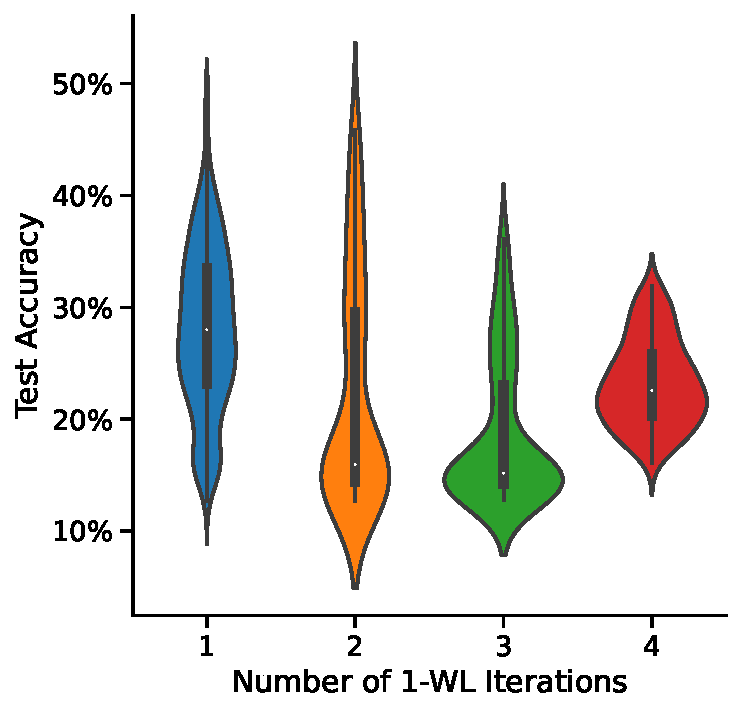
\includegraphics[width=\textwidth]{Figures/k_wl_violin_ENZYMES.pdf}
        \caption{\scriptsize\enzymes}
	\end{subfigure}
	\hfill
	\begin{subfigure}[b]{0.19\textwidth}
		\centering
		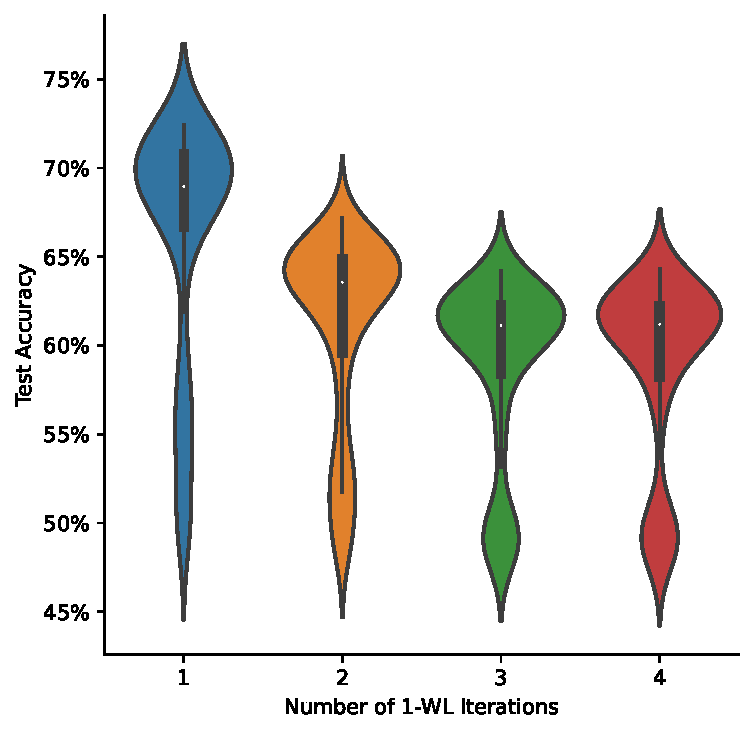
\includegraphics[width=\textwidth]{Figures/k_wl_violin_IMDB-BINARY.pdf}
        \caption{\scriptsize\imdb}
	\end{subfigure}
	\hfill
	\begin{subfigure}[b]{0.19\textwidth}
		\centering
		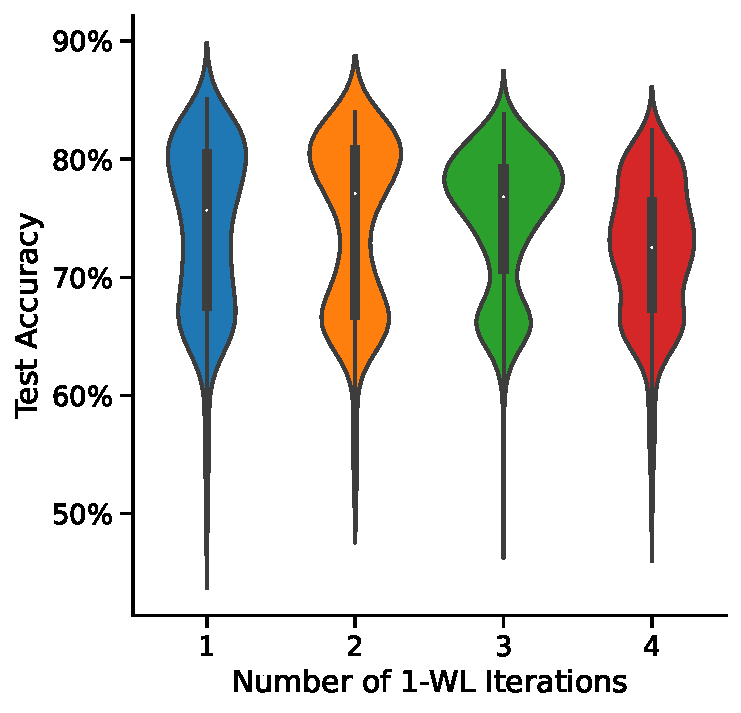
\includegraphics[width=\textwidth]{Figures/k_wl_violin_MUTAG.pdf}
        \caption{\scriptsize\mutag}
	\end{subfigure}
	\hfill
	\begin{subfigure}[b]{0.19\textwidth}
		\centering
		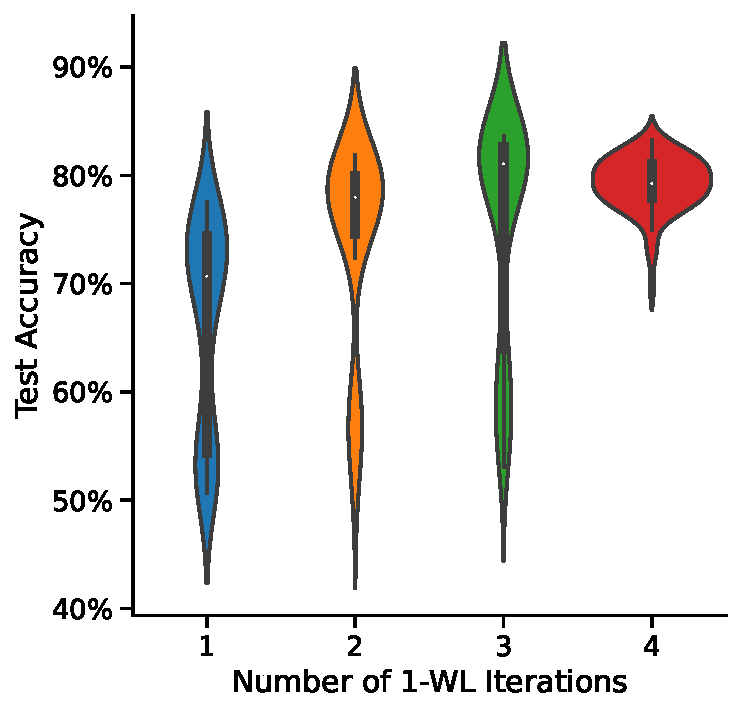
\includegraphics[width=\textwidth]{Figures/k_wl_violin_NCI1.pdf}
        \caption{\scriptsize\nci}
	\end{subfigure}
	\hfill
	\begin{subfigure}[b]{0.19\textwidth}
		\centering
		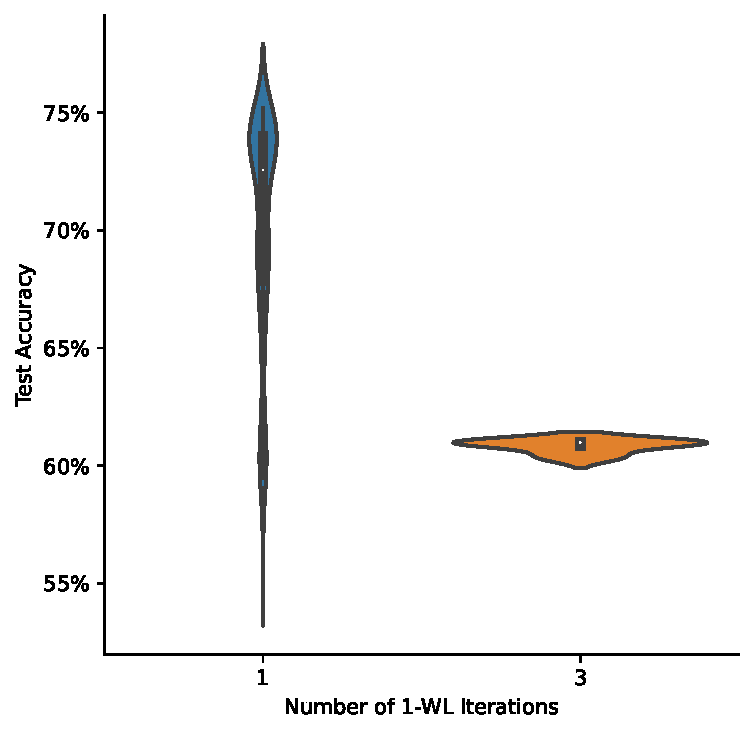
\includegraphics[width=\textwidth]{Figures/k_wl_violin_PROTEINS.pdf}
        \caption{\scriptsize\proteins}
	\end{subfigure}
	\par\bigskip
	\begin{subfigure}[b]{0.19\textwidth}
		\centering
		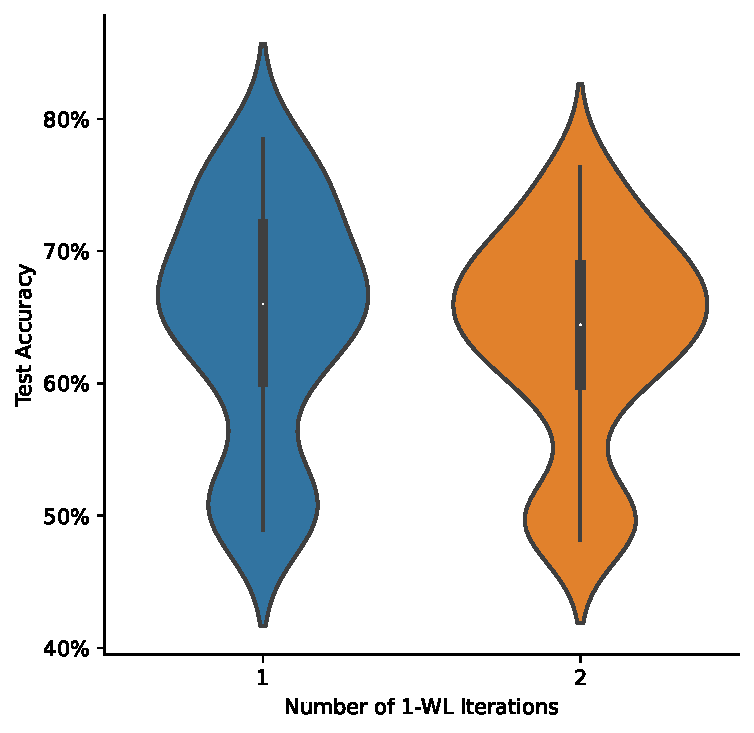
\includegraphics[width=\textwidth]{Figures/k_wl_violin_REDDIT-BINARY.pdf}
        \caption{\scriptsize \reddit}
	\end{subfigure}
	\hfill
	\begin{subfigure}[b]{0.19\textwidth}
		\centering
		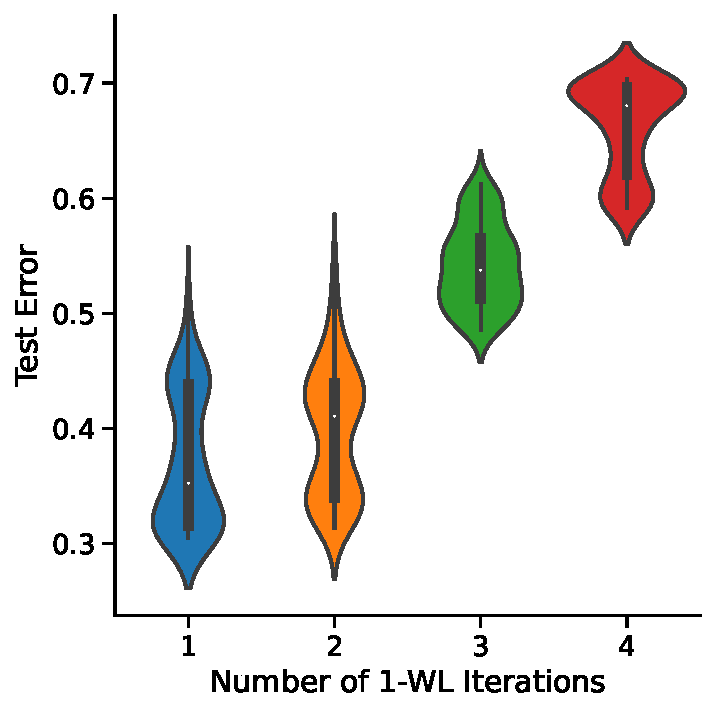
\includegraphics[width=\textwidth]{Figures/k_wl_violin_Alchemy10K.pdf}
        \caption{\scriptsize\textsc{Alchemy (10k)}}
	\end{subfigure}
	\hfill
	\begin{subfigure}[b]{0.19\textwidth}
		\centering
		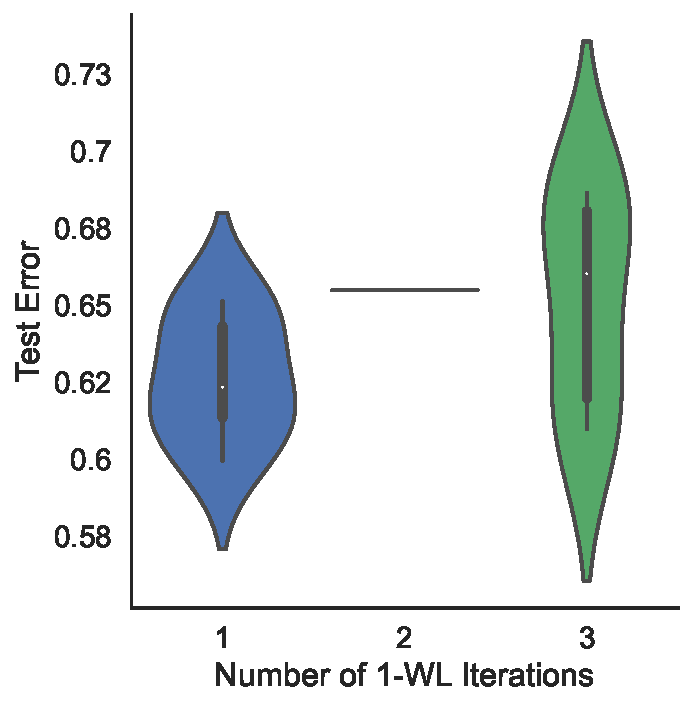
\includegraphics[width=\textwidth]{Figures/k_wl_violin_Alchemy.pdf}
        \caption{\scriptsize\textsc{Alchemy}}
	\end{subfigure}
	\hfill
	\begin{subfigure}[b]{0.19\textwidth}
		\centering
		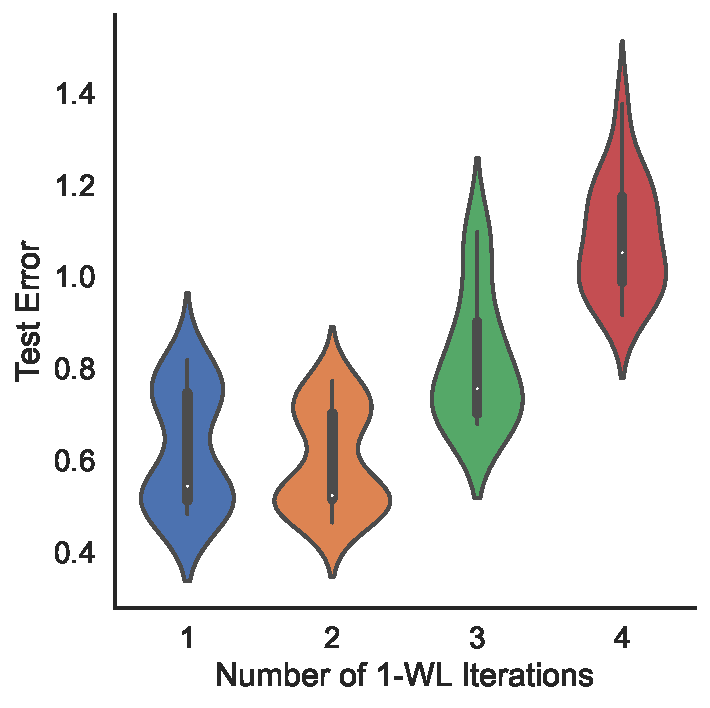
\includegraphics[width=\textwidth]{Figures/k_wl_violin_Zinc 10k.pdf}
        \caption{\scriptsize\textsc{Zinc (10k)}}
	\end{subfigure}
	\hfill
	\begin{subfigure}[b]{0.19\textwidth}
		\centering
		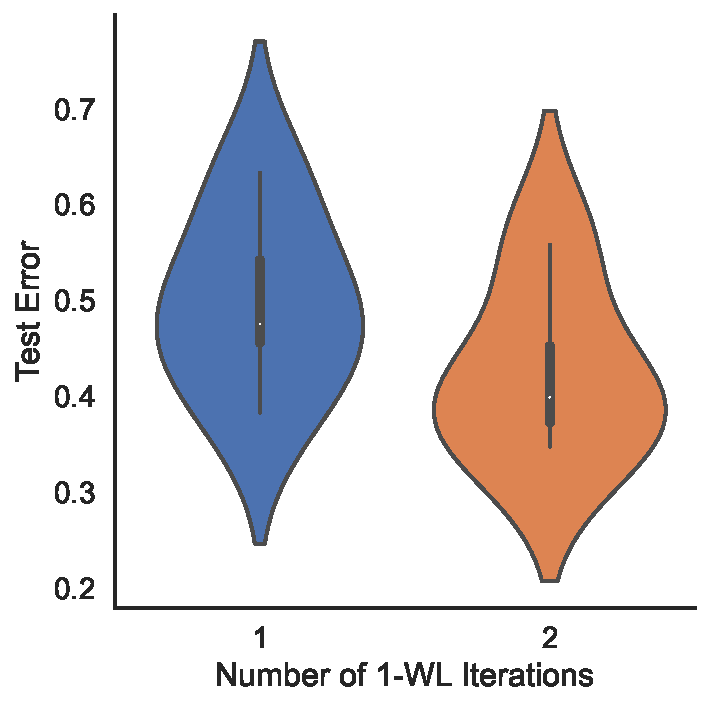
\includegraphics[width=\textwidth]{Figures/k_wl_violin_Zinc.pdf}
        \caption{\scriptsize\textsc{Zinc}}
	\end{subfigure}
	\caption{Impact on performance by the number of itertations of the \wl alogirhtm.}
	\label{fig:k_wl_dependence}
\end{figure}

In general, the results indicate that the performance of \wlnn models tends to improve as the number of \wl iterations decreases, except for the \nci and \zinc datasets. 

Notably, for \nci, the optimal number of iterations coincides with the number of \wl iterations needed for the maximum achievable accuracy (refer to \cref{tab:max_accuracies}). This correlation holds for all other classification datasets, except for \mutag. However, the behavior observed in \mutag can potentially be attributed to the fact that according to the introduced taxonomy (\cite{Liu2022}) in Section \ref{sec:datasets}, \mutag can be effectively solved by simply replacing its node features with an encoding of the node degree. Since the first iteration of the \wl alogirhtm is efficiently an encoding of the node degree, this might explain the observed pattern.

Interpreting the results of the \textsc{Zinc} dataset is more complex and somewhat peculiar. While the smaller subset of the dataset, \textsc{Zinc10K}, clearly indicates that fewer \wl iterations yield better results, the overall \textsc{Zinc} dataset suggests the opposite. This discrepancy could be attributed to the limited number of runs conducted on the entire dataset, which were restricted due to scalability and time constraints. Therefore, these results should be interpreted with caution.

In conclusion, reducing the number of \wl iterations leads to improved generability and overall better performance of the models, with the clear exception of \nci. However, as our results indicate, most \wlnn models achieve optimal performance when employing only a single iteration of the \wl algorithm, which is essentially equivalent to encoding the node degree. This observation demonstrates that \wlnn models do not require the full expressiveness of the \wl algorithm to achieve comparable performance to \gnn models, which raises the question of whether \gnn models, despite their theoretical ability to be highly expressive, also tend to rely primarily on node degree information for computation. We will explore this question in the following section.

\subsection{Difference in Learning Behavior between \gnn and \wlnn Models}
The learning behavior of \wlnn models presents a unique challenge due to the expressiveness of the \wl algorithm, which directly impacts their performance. Compared to \gnn models, \wlnn models exhibit a significant discrepancy between their training and test performance. While it is common to observe higher training performance than testing performance in various machine learning applications, this discrepancy is particularly pronounced in our evaluation of the \wlnn models.

\cref{fig:performance_diff} visually represents the difference in performance between the training and testing performance for both \wlnn and \gnn models across all classification datasets. Different quantiles from the best-performing models were considered, ranging from the top \perc{1} to the top \perc{100}. Each bar in the graph represents the mean difference between training accuracy and test accuracy for the respective quantile of runs. \wlnn models are depicted in blue, while \gnn models are represented in orange. In comparison, shorter or negative bars indicate better generalization where the performance on the training set aligns more closely with the testing set. The black line in each bar represents the standard error.

\begin{figure}[!b]
	\begin{subfigure}[b]{0.3\textwidth}
		\centering
		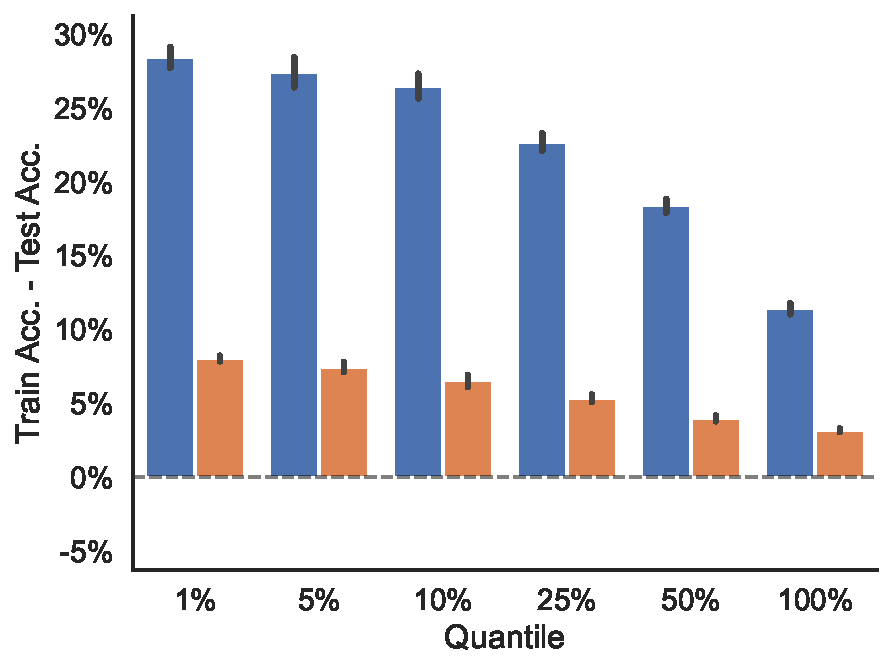
\includegraphics[width=\textwidth]{Figures/train_test_diff_ENZYMES.pdf}
		\vspace*{-4ex} 
		\caption{\enzymes}
	\end{subfigure}
	\hfill
	\begin{subfigure}[b]{0.3\textwidth}
		\centering
		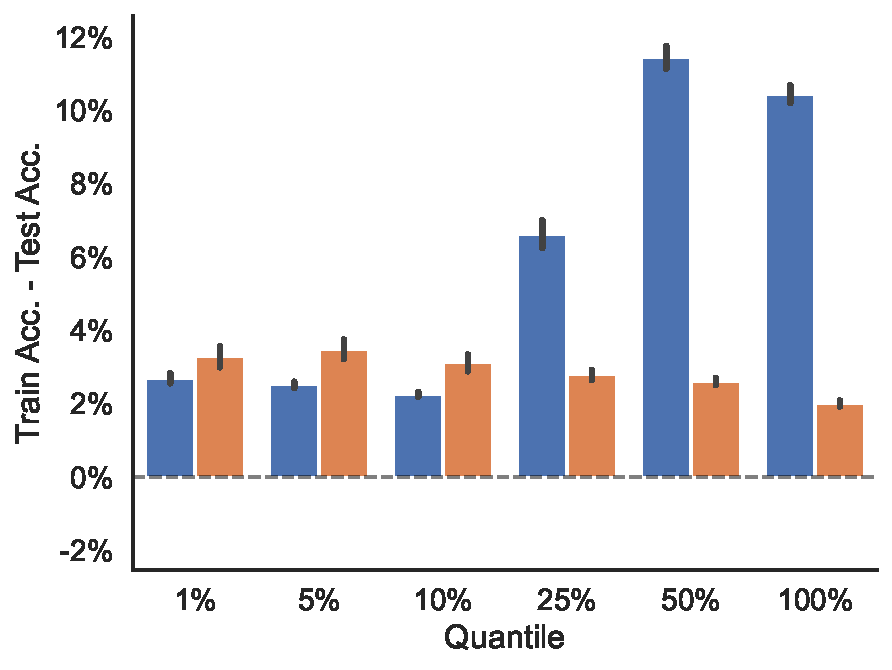
\includegraphics[width=\textwidth]{Figures/train_test_diff_IMDB-BINARY.pdf}
		\vspace*{-4ex} 
		\caption{\imdb}
	\end{subfigure}
	\hfill
	\begin{subfigure}[b]{0.3\textwidth}
		\centering
		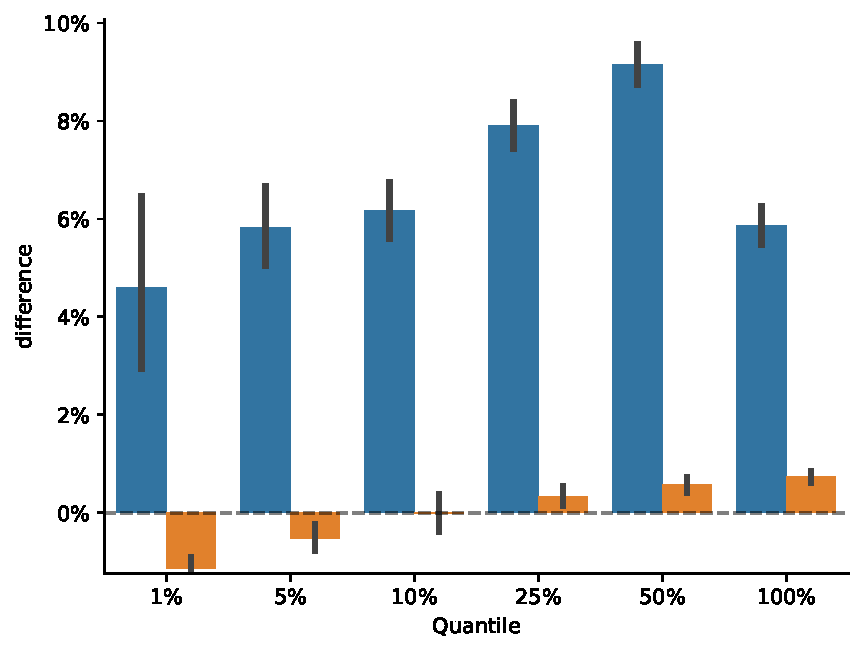
\includegraphics[width=\textwidth]{Figures/train_test_diff_MUTAG.pdf}
		\vspace*{-4ex} 
		\caption{\mutag}
	\end{subfigure}
	\par\bigskip
	\begin{subfigure}[b]{0.3\textwidth}
		\centering
		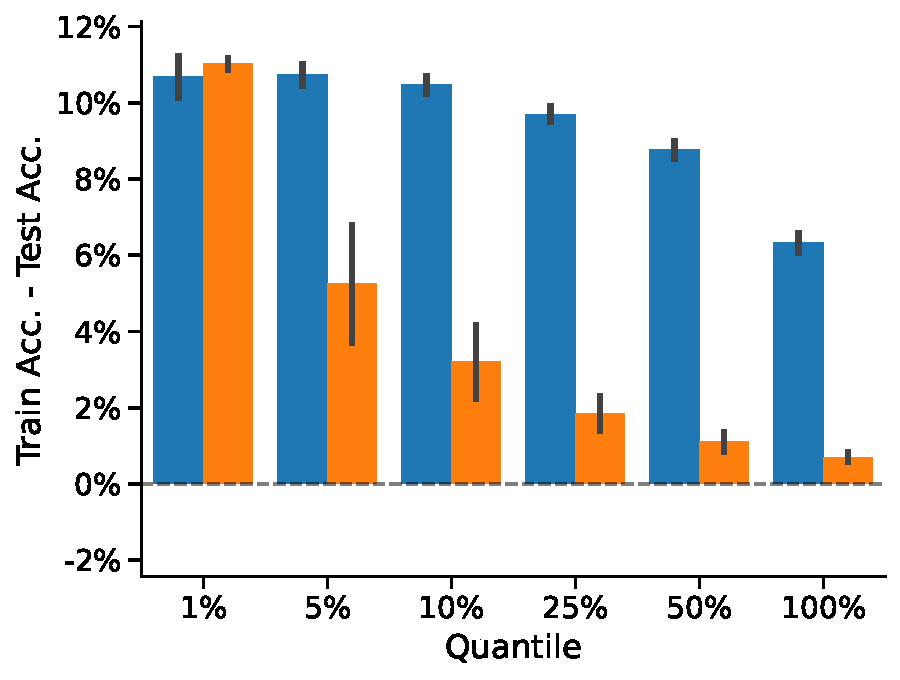
\includegraphics[width=\textwidth]{Figures/train_test_diff_NCI1.pdf}
		\vspace*{-4ex} 
		\caption{\nci}
	\end{subfigure}
	\hfill
	\begin{subfigure}[b]{0.3\textwidth}
		\centering
		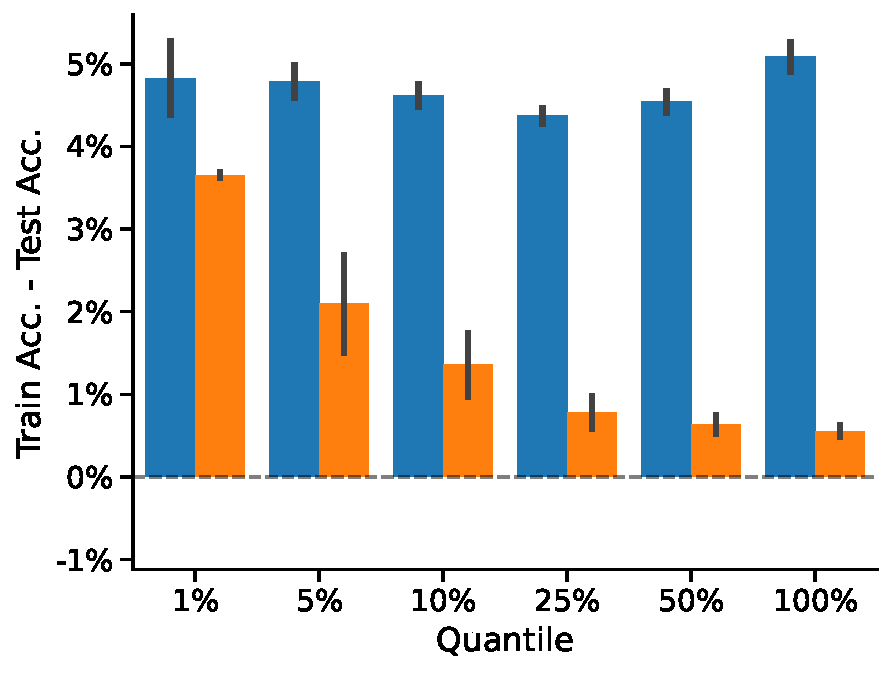
\includegraphics[width=\textwidth]{Figures/train_test_diff_PROTEINS.pdf}
		\vspace*{-4ex} 
		\caption{\proteins}
	\end{subfigure}
	\hfill
	\begin{subfigure}[b]{0.3\textwidth}
		\centering
		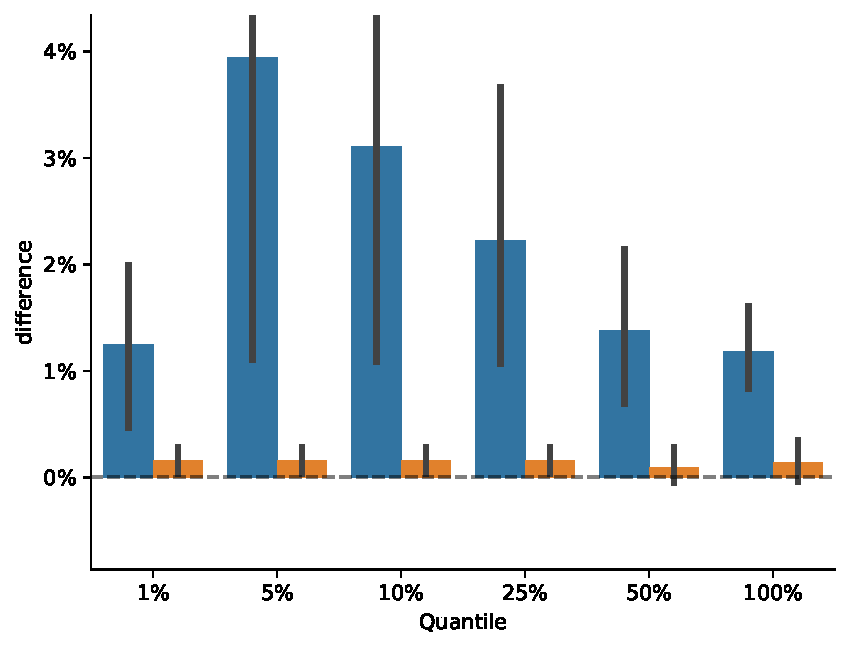
\includegraphics[width=\textwidth]{Figures/train_test_diff_REDDIT-BINARY.pdf}
		\vspace*{-4ex} 
		\caption{\reddit}
	\end{subfigure}
	\centering
	\begin{subfigure}[b]{0.3\textwidth}
		\centering
		
\includegraphics[width=\textwidth]{Figures/train_test_diff_legend.pdf}
		\vspace*{-4ex} 
	\end{subfigure}
	\caption{Mean difference of the classification accuracies of the training and testing set for each dataset. In detail, we grouped by different quantiles of the best performing models and the type of the model.}
	\label{fig:performance_diff}
\end{figure}

Upon analyzing \cref{fig:performance_diff}, it reveals that \wlnn models exhibit more significant overfitting than \gnn models, especially on datasets such as \enzymes, \mutag, \proteins, and \reddit. For instance, in the case of \enzymes, the top \perc{1} of best-performing \wlnn models display, on average, a \perc{27} higher training accuracy than their test accuracy, highlighting the extreme extent of overfitting in \wlnn models.

While \gnn models also experience some overfitting, primarily observed in the \nci dataset, it is not as prevalent across all datasets and not as dramatic as in the case of \wlnn models. Moreover, in datasets like \mutag or \reddit, \gnn models demonstrate superior generalization capability. In these cases, the mean difference in performance is close to \perc{0}, and in the case of Mutag, it is even negative, which indicates that the tested \gnn models were able to learn general patterns in these datasets rather than simply memorizing the data.

However, this raises the question as to why \wlnn models exhibit such dramatic overfitting. We hypothesize that the expressiveness of the \wl algorithm leads to the computation of highly detailed colorings of the \wlnn's input graphs, such that the models simply memorizes these.

To gain insight into the algorithm's expressiveness, we calculated the ratio of unique colors to the total number of possible colors for each classification dataset. For example, the \enzymes dataset consists of 600 graphs with a total of 19\,580 nodes. After a single iteration of the \wl algorithm, all colorings consist of only 231 unique colors, accounting for less than \perc{0.01} of the total number of possible unique colors (the total number of nodes). However, after two iterations, this number has already increased to 10\,416, comprising \perc{53.2} of the total available colors. This example demonstrates the significant expressiveness of the colorings after just a few iterations.

\begin{figure}[!htb]
	\centering
	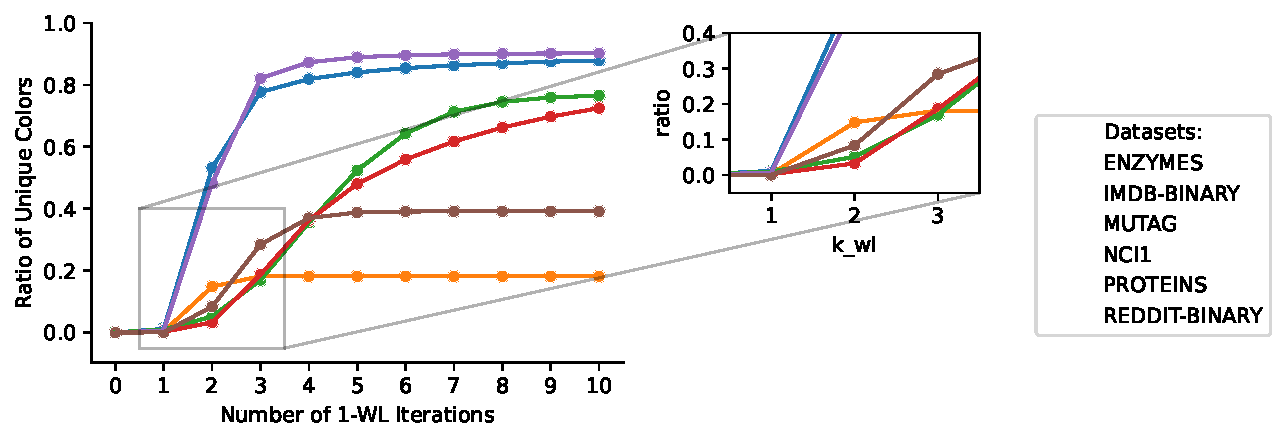
\includegraphics[width=0.975\textwidth]{Figures/wl_unique_colors.pdf}
	\caption{Overview of the ratio of unique colors used by the \wl algorithm when applied for a specified number of iterations for each dataset. The ratios are computed using each dataset's total number of nodes as the maximum number of unique colors that could appear in all colorings.}
	\label{fig:wl_unique_colors}
\end{figure}

\cref{fig:wl_unique_colors} illustrates the ratio of unique colors used compared to the total possible number of unique colors (total number of nodes in each dataset). As expected due to the convergence behavior of the \wl algorithm, each ratio convergence at some point. However, the ratios rise rapidly and dramatically for all datasets initially, indicating the strong expressiveness of the algorithm for already small numbers of iterations. Even a relatively small ratio, such as approximately \perc{10}, signifies a significant number of unique colors in the colorings computed by the \wl algorithm. It is important to consider the scale of the datasets when interpreting these ratios. For example, the \mutag dataset consists of approximately 3\,000 nodes, while the \enzymes and \imdb datasets contain around 20\,000 nodes each. The \proteins dataset reaches 43\,000 nodes, followed by the \nci dataset with 122\,000 nodes, and finally, the \reddit dataset with a staggering 859\,000 nodes. For a comprehensive overview of the datasets and their sizes, please refer to \cref{tab:overview_datasets}, and for detailed information on the unique color count, also including the regression datasets and their different splits, consult \cref{tab:unique_colors} in the Appendix.

Furthermore, it is important to note that the colors assigned by the \wl algorithm have no inherent structural connection between them. Even if two nodes are colored with two distinct integers that are close together, it does not imply any similarity between them. While our experiments use an implementation of the \wl algorithm that assigns each node the smallest unused color, a meaningful connection about the distance of colors is still absent due to shuffling the dataset and applying the \wl algorithm for a fixed number of iterations.

To investigate the impact of the number of \wl iterations on overfitting, we plotted \cref{fig:performance_diff_wlnn}, which focuses solely on \wlnn models and compares the different numbers of \wl iterations. Across all classification datasets, it is evident that the overfitting behavior becomes more substantial when increasing the number of \wl iterations. This finding supports our belief that the explosive increase in the number of unique colors is the primary reason for the observed overfitting behavior. In the case of \enzymes, with an increased number of \wl iterations, the average training accuracy is over \perc{60} higher than the test accuracy, demonstrating the worsening of the overfitting behavior.

\begin{figure}[!htb]
	\centering
	\begin{subfigure}[b]{0.3\textwidth}
		\centering
		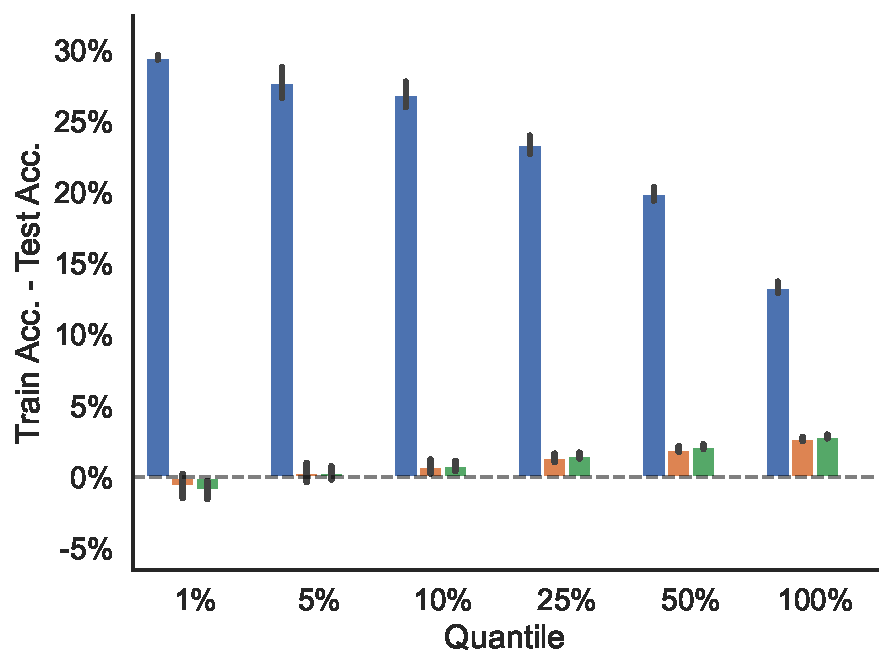
\includegraphics[width=\textwidth]{Figures/train_test_diff_k_wl_ENZYMES.pdf}
		\vspace*{-4ex} 
		\caption{\enzymes}
	\end{subfigure}
	\hfill
	\begin{subfigure}[b]{0.3\textwidth}
		\centering
		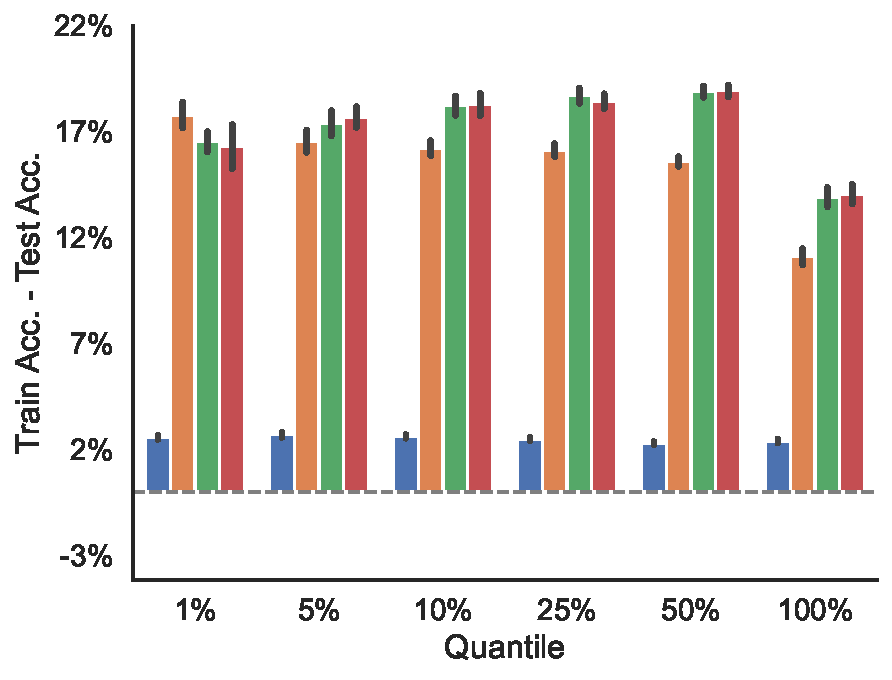
\includegraphics[width=\textwidth]{Figures/train_test_diff_k_wl_IMDB-BINARY.pdf}
		\vspace*{-4ex} 
		\caption{\imdb}
	\end{subfigure}
	\hfill
	\begin{subfigure}[b]{0.3\textwidth}
		\centering
		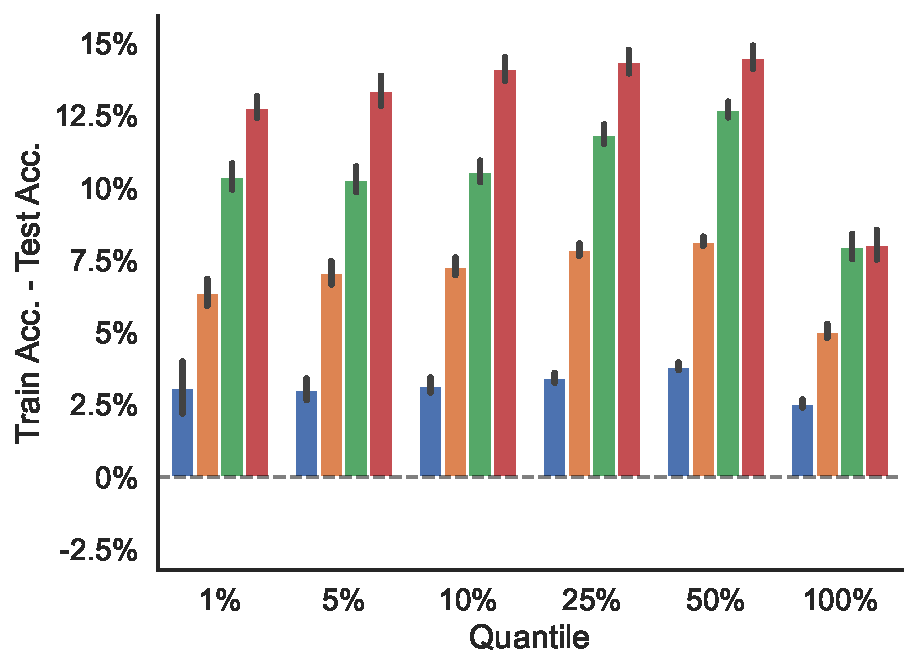
\includegraphics[width=\textwidth]{Figures/train_test_diff_k_wl_MUTAG.pdf}
		\vspace*{-4ex} 
		\caption{\mutag}
	\end{subfigure}
	\par\bigskip
	\begin{subfigure}[b]{0.3\textwidth}
		\centering
		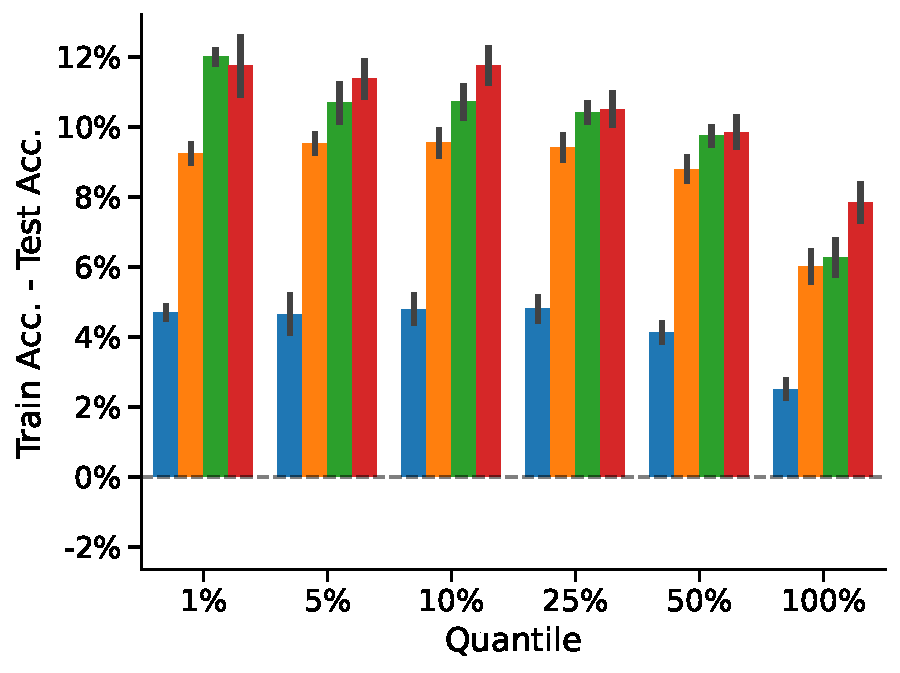
\includegraphics[width=\textwidth]{Figures/train_test_diff_k_wl_NCI1.pdf}
		\vspace*{-4ex} 
		\caption{\nci}
	\end{subfigure}
	\hfill
	\begin{subfigure}[b]{0.3\textwidth}
		\centering
		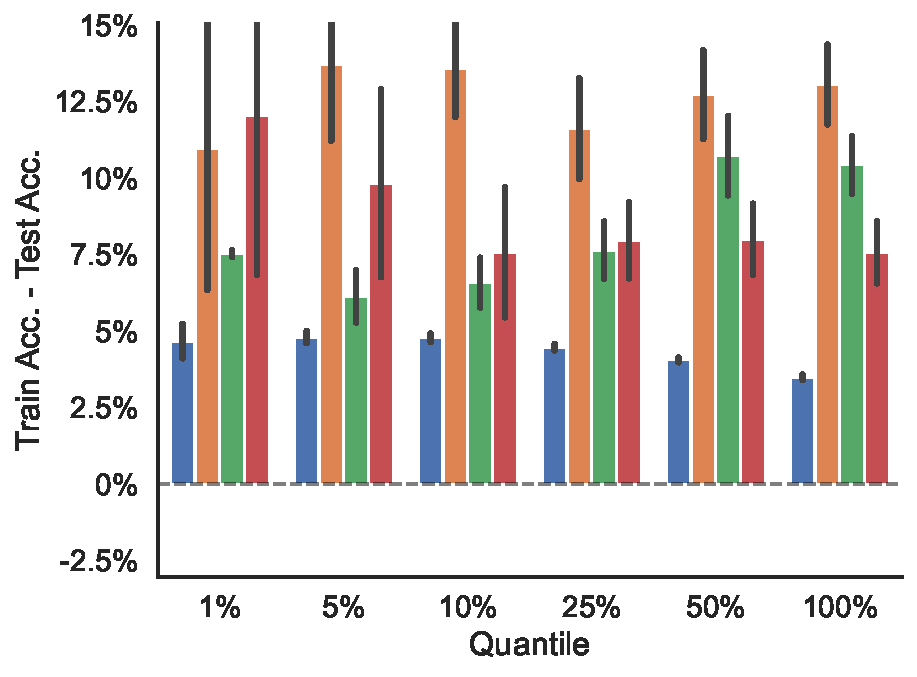
\includegraphics[width=\textwidth]{Figures/train_test_diff_k_wl_PROTEINS.pdf}
		\vspace*{-4ex} 
		\caption{\proteins}
	\end{subfigure}
	\hfill
	\begin{subfigure}[b]{0.3\textwidth}
		\centering
		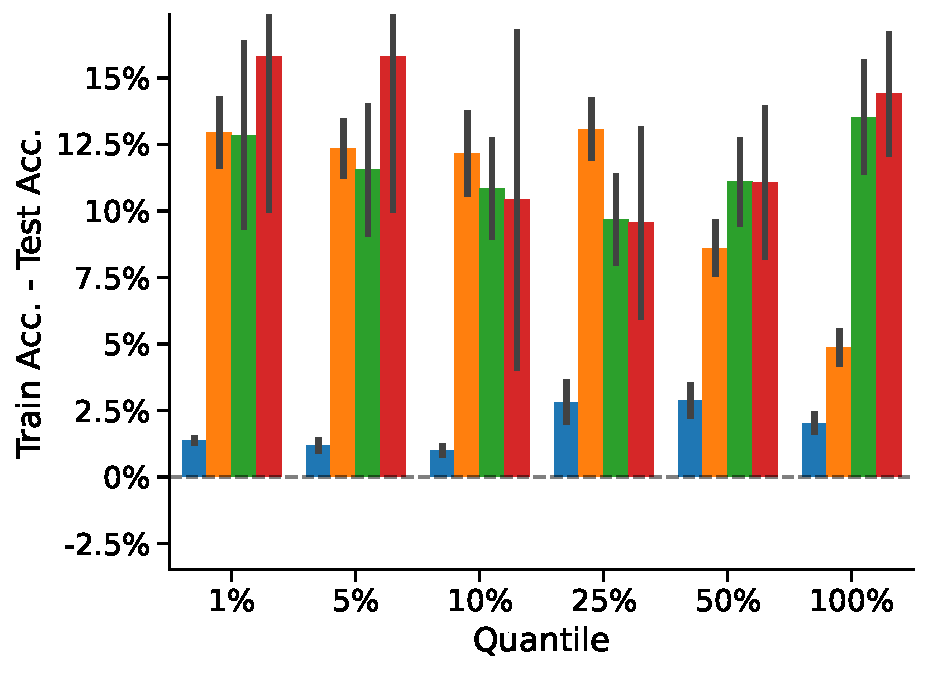
\includegraphics[width=\textwidth]{Figures/train_test_diff_k_wl_REDDIT-BINARY.pdf}
		\vspace*{-4ex} 
		\caption{\reddit}
	\end{subfigure}
	\begin{subfigure}[b]{0.3\textwidth}
		\centering
		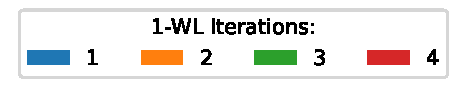
\includegraphics[width=\textwidth]{Figures/train_test_diff_k_wl_legend.pdf}
		\vspace*{-4ex} 
	\end{subfigure}
	\caption{Mean difference in the classification accuracy of the training and test sets achieved by all \wlnn models for each dataset. In detail, we grouped the best models according to different quantiles and the number of iterations of the \wl algorithm used by each model.}
	\label{fig:performance_diff_wlnn}
\end{figure}

In conclusion, our analysis reveals that \wlnn models exhibit optimal generalization when limited to one iteration of the \wl algorithm. Increasing the number of iterations leads to a significant overfitting behavior. This insight indicates that the expressiveness of the \wl algorithm surpasses the requirements for effective learning. In comparison, \gnn models excel in learning and representing graph structures in a more generalized manner. The observation that a single iteration of the \wl algorithm leads to the best generalization also aligns with the results from the previous section, where the models achieving the highest accuracy on the test set also utilized only a single iteration of the \wl algorithm (except for the \nci dataset). This observation raises an intriguing question: Do \gnns also attempt to compute a similarly expressive representation of all graphs, akin to a single iteration of the \wl algorithm? We will explore this question in the following section.

\FloatBarrier
\subsection{Approximating \wl Coloring: Investigating \gnn Node Representations}
This section will explore the node features computed by a \gnn. Specifically, we will analyze the ability of \gnns to approximate the coloring computed by a single iteration of the \wl algorithm.

To visualize the approximation capabilities of the best-performing \gnn models on various classification datasets, refer to Figure \ref{fig:gnn_approx}. The visualization consists of a pair of color-coded matrices for each dataset, where each pair represent a single randomly drawn graph from the test set of the respective \gnn model. The left matrix illustrates the distance matrix of the node representations computed by the \gnn model for each pair of nodes $i$ and $j$. In contrast, the right matrix represents the distances of the colorings generated by a single iteration of the \wl algorithm. The distances are measured using the Euclidean distance and then normalized between 0 and 1 for the \gnn matrix. While the distances between the \wl coloring are either $0$ (for nodes with the same color) or $1$ (for nodes with different colors) since the colorings produced by the \wl algorithm are discrete and do not encode any information in their distances. Further, we computed the similarity between both matrices by using their absolute difference and average these, resulting in a single value represented as the Mean Absolute Error (MAE). The MAE, along with its standard deviation and the index of the graph in the datasets, is included on the right side of the \wl distance matrix.

\begin{figure}[!htb]
	\centering
	\begin{subfigure}[b]{0.49\textwidth}
		\centering
		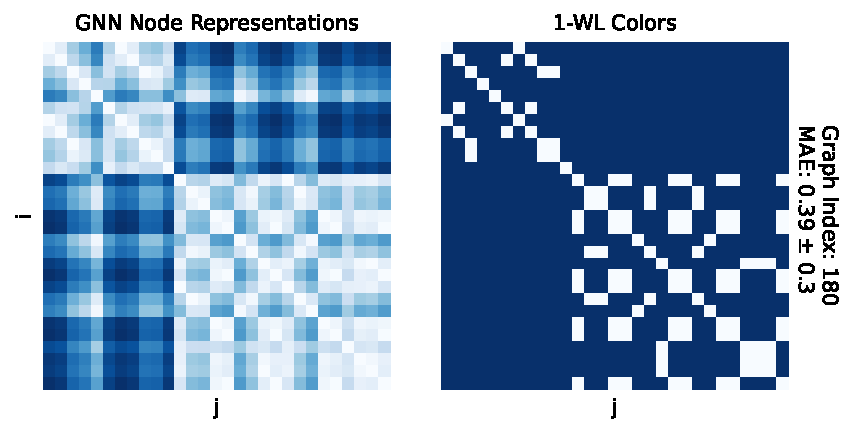
\includegraphics[width=\textwidth]{Figures/heatmaps_ENZYMES_single.pdf}
		\vspace*{-5ex} 
        \caption{\enzymes}
	\end{subfigure}
	\hfill
	\begin{subfigure}[b]{0.49\textwidth}
		\centering
		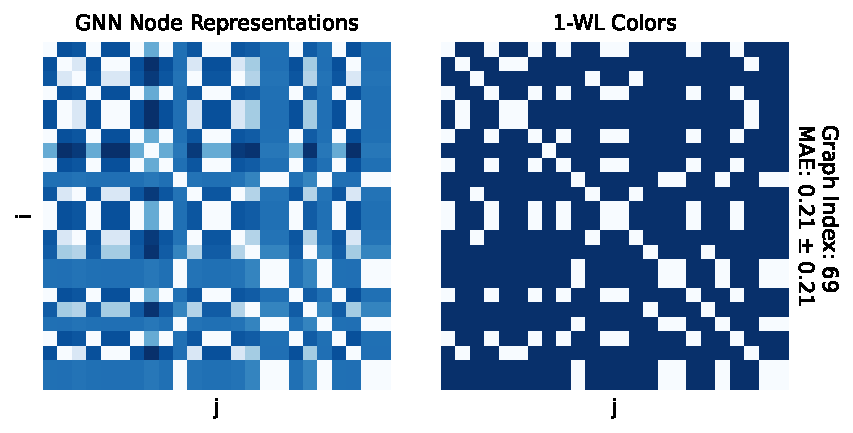
\includegraphics[width=\textwidth]{Figures/heatmaps_IMDB-BINARY_single.pdf}
		\vspace*{-5ex} 
        \caption{\imdb}
	\end{subfigure}
	\par\bigskip
	\begin{subfigure}[b]{0.49\textwidth}
		\centering
		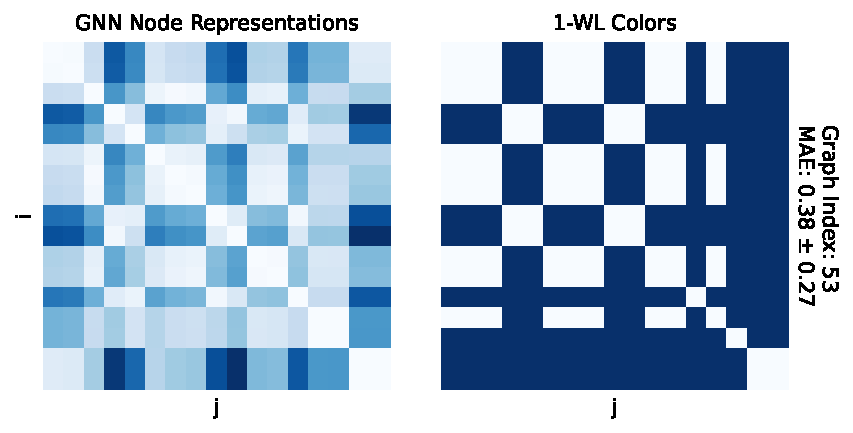
\includegraphics[width=\textwidth]{Figures/heatmaps_MUTAG_single.pdf}
		\vspace*{-5ex} 
        \caption{\mutag}
	\end{subfigure}
	\hfill
	\begin{subfigure}[b]{0.49\textwidth}
		\centering
		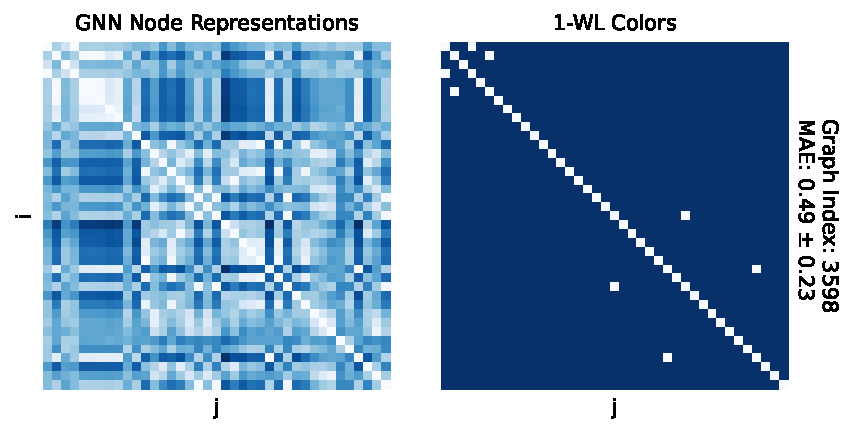
\includegraphics[width=\textwidth]{Figures/heatmaps_NCI1_single.pdf}
		\vspace*{-5ex} 
        \caption{\nci}
	\end{subfigure}
	\par\bigskip
	\begin{subfigure}[b]{0.49\textwidth}
		\centering
		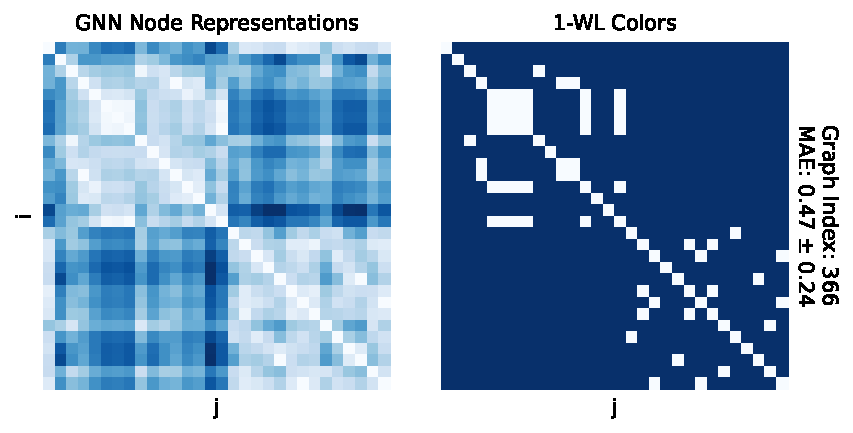
\includegraphics[width=\textwidth]{Figures/heatmaps_PROTEINS_single.pdf}
		\vspace*{-5ex} 
        \caption{\proteins}
	\end{subfigure}
	\hfill
	\begin{subfigure}[b]{0.49\textwidth}
		\centering
		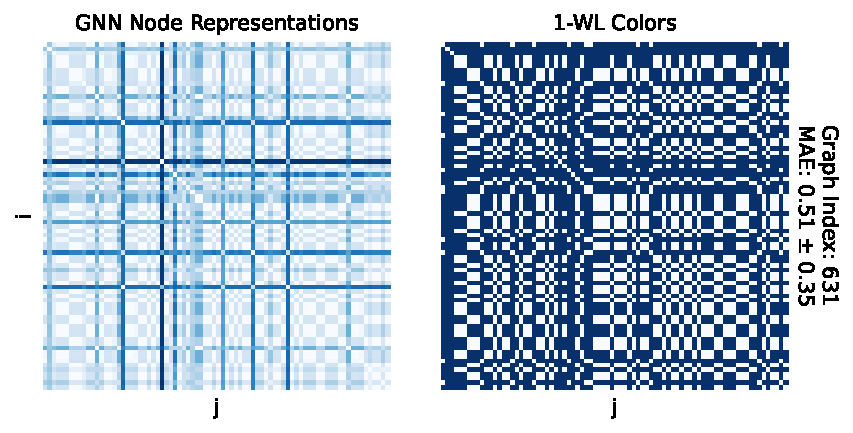
\includegraphics[width=\textwidth]{Figures/heatmaps_REDDIT-BINARY_single.pdf}
		\vspace*{-5ex}
        \caption{\reddit}
	\end{subfigure}
	\par\bigskip
	\begin{subfigure}[t]{0.6\textwidth}
		\centering
		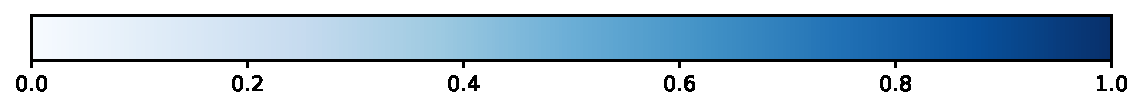
\includegraphics[width=\textwidth]{Figures/colorbar.pdf}
	\end{subfigure}
	\caption{Visualizing the performance of the best-performing \gnn models of each dataset in approximating node colors computed by the \wl algorithm after running for one iteration. Here we randomly sampled a single graph for each dataset and visualized the approximation performance.}
	\label{fig:gnn_approx}
\end{figure}

The visualization shows that the \gnn representations already provide convincing approximations of the patterns observed in the \wl algorithm's matrix. However, it is important to note that these results are based on a single randomly selected graph from each model's test set. To obtain a more comprehensive understanding of the approximation capabilities, we repeated this process for each dataset using ten randomly selected graphs from the test set of the respective \gnn model, refer to \cref{fig:gnn_approx_enzymes,fig:gnn_approx_imdb,fig:gnn_approx_mutag,fig:gnn_approx_nci_1,fig:gnn_approx_nci_3,fig:gnn_approx_proteins,fig:gnn_approx_reddit} in the Appendix.

Before diving deeper into analyzing the approximation capabilities, it is crucial to highlight the significant difference between the node representations computed by a \gnn and the colors computed by the \wl algorithm. Unlike the discrete colors with no order relation calculated by the \wl algorithm, the representations computed by each \gnn model are multidimensional and continuous. This difference makes a perfect approximation of the \wl colorings challenging, as determining when two node representations are similar is not as straightforward as in the discrete \wl case. In the visualization, we avoided making this decision by uniformly normalizing the distances between 0 and 1 and using a continuous color bar for color coding similar nodes. However, to comprehensively evaluate each dataset entirely, we employed two approaches for tackling this problem: 1) evaluating the approximation using a threshold value for similarity (continuous approximation) and 2) translating the values into discrete distances and using the F1 score for assesing similarity (discrete approximation).

\begin{figure}[!htb]
	\centering
	\begin{subfigure}[t]{0.39\textwidth}
		\centering
		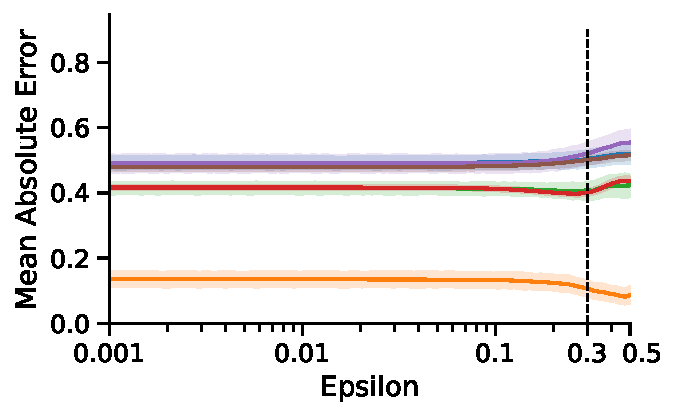
\includegraphics[width=\textwidth]{Figures/global_error_1_b.pdf}
		\caption{Continous Approximation}
		\label{fig:approx_error}
	\end{subfigure}
	\hfill
	\begin{subfigure}[t]{0.39\textwidth}
		\centering
		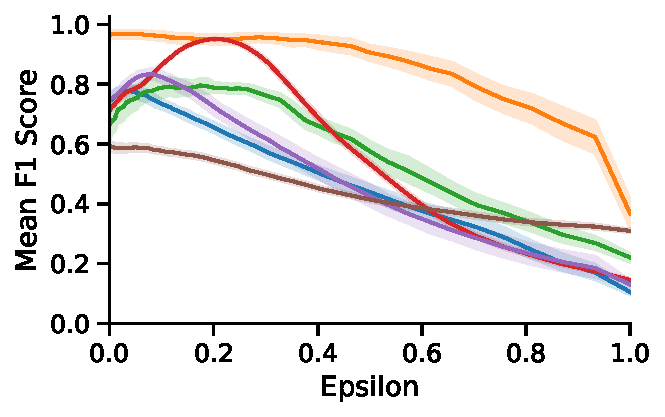
\includegraphics[width=\textwidth]{Figures/global_error_2_b.pdf}
		\caption{Discrete Approximation}
		\label{fig:approx_error_f1}
	\end{subfigure}
	\hfill
	\begin{subfigure}[t]{0.2\textwidth}
		\centering
		\raisebox{22pt}{
			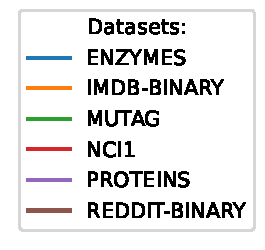
\includegraphics[width=\textwidth]{Figures/global_error_legend.pdf}
		}
	\end{subfigure}
	\caption{Results obtained by using the proposed evaluation procedures to assess the ability of \gnns to approximate \wl colorings.}
	\label{fig:approx_eval}
\end{figure}

In the first procedure, two node representations are considered similar if their Euclidean distance is less than a threshold value, $\epsilon$. Additionally, we consider the distances perfectly separable if their distance is greater or equal to $1 - \epsilon$. In detail, we modify the \gnn distance matrix for every graph such that all distances less than $\epsilon$ are set to $0$, all distances greater or equal to $1 - \epsilon$ to $1$, otherwise the original distance is preserved. Afterward, we compute, as before, the MAE between each \gnn matrix and the \wl color matrix and average all values for the entire dataset in a single MAE value in the end. We tested this procedure with various threshold values $\epsilon \in [0, 0.5)$. See Figure \ref{fig:approx_error} for an illustration of the MAE for all classification datasets. Since the distances are normalized, a higher $\epsilon$ value indicates classifying the majority of distances as negligible. As a result, the values of interest are small, which is why a logarithmic scale is used for the x-axis.

The second procedure aims to transform the regression-like values into a classification task by introducing a threshold value, $\epsilon$, which maps distances between two node representations to a discrete value. Distances less than $\epsilon$ are classified as 0, while distances greater than or equal to $\epsilon$ are classified as 1. This process generates a distance matrix with discrete values, and the F1 score is used to evaluate the approximation capability of this newly devised matrix to the \wl coloring distance matrix. The process is repeated for each graph in a dataset, and the average F1 score is calculated as the final evaluation metric. Since the number of node pairs distinguished by the \wl algorithm differs from the number of nodes assigned the same color, an imbalance between the two labels exists. To counter any biases due to this imbalance, the F1 score is computed with macro weighting. Figure \ref{fig:approx_error_f1} provides a visualization of the results for each classification dataset.

Analyzing the figures, it becomes apparent that the approximation of the \wl coloring is not perfect, as indicated by the relatively high MAE and the varying F1 scores for different datasets, with the clear exception of the \imdb dataset. Since the \imdb and \reddit datasets lack node features, we initialized their features using the common procedure of encoding their node degrees. Since the coloring computed by a single iteration of the \wl algorithm is an encoding of the node degree, this explains the good performance of the \imdb dataset. However, due to the large size of the \reddit dataset and its graphs, a one-hot encoding of the node degree is not practical. Instead, a continuous, one-dimensional node degree encoding is employed that uniformly maps a node degree into the range $[-1, 1]$. This difference in encoding is evident in the significant performance gap between these datasets in the approximation evaluation.

Interestingly, the MAE remains constant for $\epsilon$ values up to $0.3$, as depicted in Figure \ref{fig:approx_error}, suggesting that the \gnn models tend to map nodes with different values far away from each other and vice versa for small values. This observation aligns with the low standard deviation values, indicating consistent behavior across all graphs. Moreover, to strengthen this insight, we plotted the frequency of distances that appears in the \gnn distance matrices for each dataset. We calculated the frequency by creating ten uniformly, non-overlapping intervals between $0$ and $1$ and counted the number of distances that fall in this interval for each. Interestingly, we do not see an intense concentration of any distances in any of the intervals such that we can out rule any bias when analyzing the threshold values. Since $0.3$ is already a considerable threshold for removing distances, we infer that the \gnns compute a coloring that incorporates essential information from the \wl coloring while leaving out less important information. The visual representations show that the distances between nodes exhibit similar patterns as the coloring produced by the \wl algorithm, although not as perfect. Since the \gnn models perform nearly as well as most of the \wlnn models in terms of their accuracy performance, we conclude that \gnns are able to learn a more efficient encoding of the graph structure that holds the most important structural information of the \wl coloring.

\begin{figure}[!htb]
	\centering
	\begin{subfigure}[t]{0.45\textwidth}
		\centering
		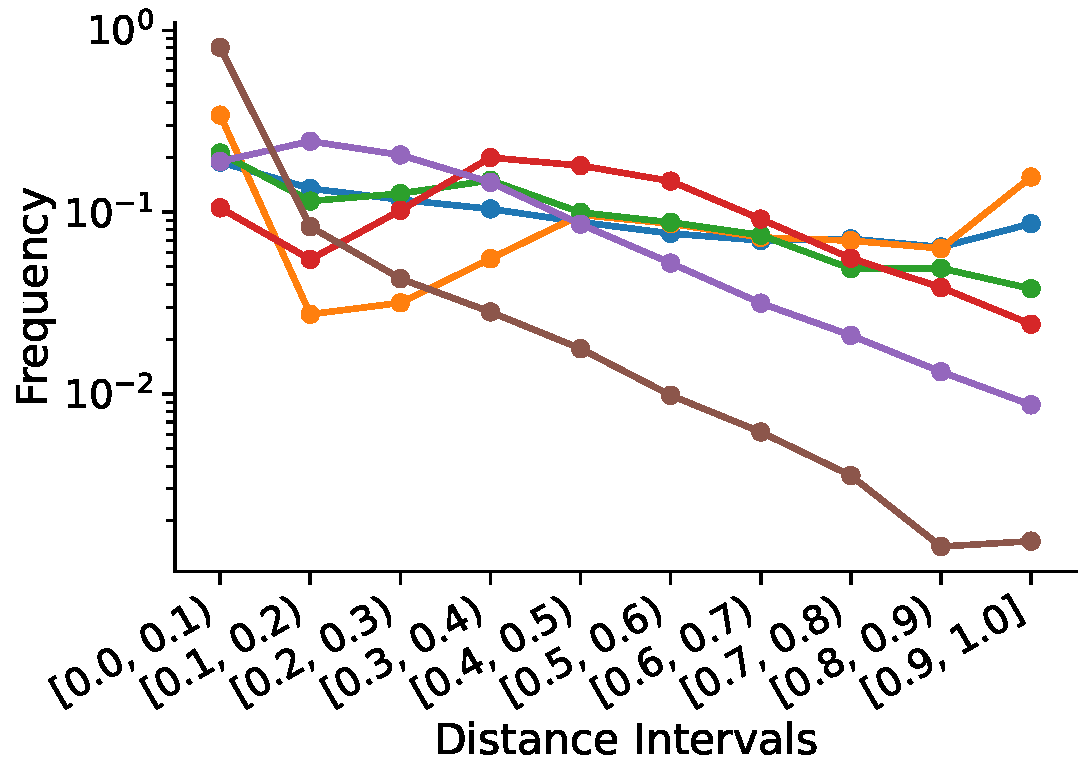
\includegraphics[width=\textwidth]{Figures/global_error_distances.pdf}
	\end{subfigure}
	\begin{subfigure}[t]{0.2\textwidth}
		\centering
		\raisebox{45pt}{
			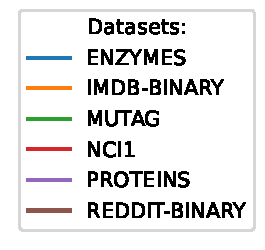
\includegraphics[width=\textwidth]{Figures/global_error_legend.pdf}
		}
	\end{subfigure}
	\caption{Visualization of the frequency of the distance between node pairs in the representation computed by the best-performing \gnn model. In detail, we divided the distance space into ten non-overlapping intervals and counted the number of occurrences that fall into this interval for each dataset.}
	\label{fig:approx_error_dist}
\end{figure}

Analyzing the other procedure, we observe that each dataset has its own optimal threshold value $\epsilon$ for the F1 score. Interestingly, these optima consistently fall within a narrow range between $0.0$ and $0.2$. Moreover, most datasets achieve a high F1 score, providing further evidence for our hypothesis regarding the encoding of essential structural information. With the exception of \reddit, almost all datasets achieve a score higher than $0.77$. Notably, the \nci dataset stands out with an exceptional Mean F1 score of $0.95$ for $\epsilon = 0.2$. This result indicates that the node representations computed by the best \gnn model for \nci effectively encode the structural information captured by a single iteration of the \wl algorithm. Furthermore, considering the dataset taxonomy introduced in \cref{sec:datasets}, \nci belongs to the dataset category that encodes a substantial amount of information in their graph structures, which aligns with our findings.
It is also worth noting that \nci is the only dataset that demonstrates improved performance, in terms of accuracy, with an increased number of \wl iterations in the testing of the \wlnn models (refer to Figure \ref{fig:k_wl_dependence}). To further investigate this behavior, we explored the approximation capability of the \gnn model for the coloring computed by three iterations of the \wl algorithm specifically for the \nci dataset. The results are visualized in Figure \ref{fig:gnn_approx_nci_3} in the Appendix. However, as explained in the previous section, the number of unique colors increases significantly with an increased number of \wl iterations. This has the effect that almost all nodes in a graph need to be mapped to separable node representation, which is not the case, as we see in \cref{fig:approx_error_dist}. This limitation applies to all datasets, leading us to conclude that \gnns cannot effectively approximate a higher number of \wl iterations.

Although the \reddit dataset exhibit visually good approximation, as displayed in \cref{fig:gnn_approx} and \cref{fig:gnn_approx_reddit} in the Appendix, it performs poorly in the approximation evaluation for the entire dataset. We believe that the reason for this is due to the sheer size of the dataset, particularly the size of its graphs. While all other classification datasets have an average of approximately $30$ nodes per graph (including the regression datasets), \reddit averages $429.6$ nodes per graph. The significantly larger number of nodes causes challenges in efficiently propagating information across the graph for \gnn models. With a fixed number of message-passing layers, set to 5 for scalability and comparability, it is likely that some information is not shared with the entire graph. This issue is also present in other datasets but is more pronounced in \reddit, as indicated by the average number of nodes. \todo{!}

In conclusion, considering the similar performance of \gnn and \wlnn models and the relatively robust approximation capabilities of \gnns compared to the \wl coloring after a single iteration, we argue that \gnns can learn a more efficient encoding of this information. Given that both frameworks achieve comparable performance on all datasets in terms of accuracy, combined with the fact that most models utilize only a single iteration of the \wl algorithm or an approximation, the question arises as to whether this difference remains when pooling this information using the same pooling function. This question will be investigated in the next section.\todo{!}

\FloatBarrier
\subsection{Comparing Pooled Graph Representations: \gnn vs. \wlnn Models}
After the previous section, we observed that \gnns do not perfectly approximate the coloring calculated by the \wl algorithm. However, we hypothesized that \gnns might employ a more efficient encoding containing only essential information. To delve deeper into this, we compared the different graph representations derived after applying the respective pooling functions. To do this, we selected the best-performing \gnn and \wlnn models in terms of classification accuracy for each dataset and replaced the final \mlp with various algorithms.

\begin{table}[!htb]
	\caption{Overview of the classification accuracies achieved by the best model configuration for each dataset in percent and standard deviation. Additionally, the performance of each configuration was furhter evaluated by substituting the final \mlp with either a \textsf{SVM} utilizing a linear kernel (\textsf{SVM Linear}) or the Radial Basis Function (\textsf{SVM RBF}), as well as the \textsf{$k$-NN} classifier with different values for $k$.}
	\label{tab:pool_analysis}  
    \resizebox{.975\textwidth}{!}{ 	\renewcommand{\arraystretch}{1.05}
		\begin{tabular}{@{}c <{\enspace}@{}lcccccc@{}}	\toprule
			& \multirow{3}{*}{\vspace*{4pt}\textbf{Method}}&\multicolumn{6}{c}{\textbf{Dataset}}\\\cmidrule{3-8}
			& & {\enzymes}         &  {\imdb}      & {\mutag}           & {\nci}       & {\proteins}           & 
			{\reddit}
			\\
			\toprule
			\multirow{4}{*}{\rotatebox{90}{$\wlnn$}}
			& \textsf{MLP} & 48.3 \scriptsize	$\pm 8.1$ & \textbf{72.4} \scriptsize	$\pm 4.1$ & 85.1 \scriptsize $\pm 8.6$ & 83.6 \scriptsize	$\pm 4.1$ & \textbf{75.2} \scriptsize $\pm 3.9$ & 78.4 \scriptsize $\pm 2.7$
			\\
			& \textsf{SVM Linear} & 34.4 \scriptsize	$\pm 5.5$ & 71.2 \scriptsize	$\pm 3.9$ & 86.4 \scriptsize $\pm 8.9$	 & 83.4 \scriptsize	$\pm 2.1$ & 73.9 \scriptsize $\pm 4.1$ & 77.8 \scriptsize $\pm 2.7$
			\\
			& \textsf{SVM RBF} & 45.0 \scriptsize	$\pm 7.0$ & 72.8 \scriptsize	$\pm 4.3$ & 83.2 \scriptsize $\pm 7.5$ & 83.6 \scriptsize	$\pm 1.9$ & 75.2 \scriptsize $\pm 4.0$ & 78.3 \scriptsize $\pm 2.4$
			\\
			& \textsf{$k$-NN} &  \textbf{56.3} \scriptsize $\pm 5.8$ ($k$=$1$) & 72.3 \scriptsize $\pm 4.1$ ($k$=$11$)& \textbf{86.7} \scriptsize $\pm 7.7$ ($k$=$10$) & \textbf{83.9} \scriptsize $\pm 1.8$ ($k$=$5$)& 73.9 \scriptsize $\pm 4.1$ ($k$=$19$) & \textbf{83.2} \scriptsize $\pm 2.5$ ($k$=$13$)
			\\
			\cmidrule{2-8}
			\multirow{4}{*}{\rotatebox{90}{\gnn}}
			& \textsf{MLP} & 34.4 \scriptsize $\pm 7.0$ &  \textbf{74.7} \scriptsize $\pm 3.8$ & 84.6 \scriptsize $\pm 8.7$	 & \textbf{79.9} \scriptsize $\pm 2.2$ & 74.3 \scriptsize $\pm 5.1$ & 86.9 \scriptsize $\pm 3.2$
			\\
			& \textsf{SVM Linear} & 33.2 \scriptsize $\pm 5.9$ & 73.9 \scriptsize $\pm 4.2$ & \textbf{87.4} \scriptsize $\pm 6.8$ & 67.4 \scriptsize $\pm 2.2$ & 74.7 \scriptsize $\pm 4.2$ & 84.2 \scriptsize $\pm 2.8$
			\\
			& \textsf{SVM RBF} & 35.9 \scriptsize $\pm 6.0$ & 74.1 \scriptsize $\pm 3.9$ & 86.0 \scriptsize $\pm 7.4$ & 73.0 \scriptsize $\pm 1.9$ & 74.6 \scriptsize $\pm 4.6$ & 88.7 \scriptsize $\pm 2.4$
			\\ 
			& \textsf{$k$-NN} & \textbf{51.6} \scriptsize $\pm 7.0$ ($k$=$1$)	& 74.3 \scriptsize $\pm 4.0$ ($k$=$132$) & 88.3 \scriptsize $\pm 6.5$ ($k$=$38$) & 77.5 \scriptsize $\pm 1.7$ ($k$=$2$)& \textbf{74.9} \scriptsize $\pm 4.3$ ($k$=$27$) & \textbf{90.8} \scriptsize $\pm 1.8$ ($k$=$15$)
			\\
			\bottomrule
		\end{tabular}}                
\end{table}

Specifically, we used two different configurations of \textsf{Support Vector Machines (SVM)}: one with a linear kernel (\textsf{SVM Linear}) and another with a radial basis function (\textsf{SVM RBF}). Additionally, we employed the \textsf{$k$-Nearest-Neighbor ($k$-NN)} classifier for different values of $k$. Each algorithm was trained exclusively on the fixed output of the pooling function. To ensure fair comparisons, we froze the weights of the \gnn models and the Look-Up Table of the \wlnn models during this process to ensure no optimization of underlying parameters before pooling. This approach guarantees more comparable results across algorithms. Moreover, we maintained the same training, validation, and test split used for training and evaluating the \mlp. For a comprehensive evaluation, we summarized the accuracies and standard deviations achieved by each method, comparing them to the \mlp's performance in \cref{tab:pool_analysis}. Furthermore, in the case of the \textsf{$k$-NN} algorithm, we provided the achieved accuracy for the optimal $k$ value, including the $k$ value in the brackets. This analysis will allow us to make statements about the linear separability of the graph representations as well as how well these cluster with respect to their class labels.

Starting with the investigation of linear separability, we used the performance of \textsf{SVM Linear} as our basis of evaluation since this method learns a linear high-dimensional hyperplane to separate the graph representations optimally. The results of the \textsf{SVM RBF} serve as a baseline that shows how effectively the data will be linear separable after applying the \textsf{RBF} kernel. Therefore, if both \textsf{SVM} methods achieve similar performance, we can conclude that the graph representations are already relatively linearly separable, and there is no need for applying an additional kernel function.

Interestingly, for both \gnn and \wlnn models, the linear \textsf{SVM} performed comparably to the \mlp, with the exceptions of \enzymes for the \wlnn model and \nci for the \gnn model. In fact, \textsf{SVM Linear} even outperformed the \mlp of the \gnn model on \mutag, indicating the graph representations strong linear separability. Furthermore, since the insights were similar for both \gnn and \wlnn models, we concluded that both methods map their graph representations in such a way as to facilitate easy linear separation. Additionally, we observed that the accuracy achieved by \textsf{SVM RBF} is higher than the one of \textsf{SVM Linear}; however, this difference is negligible and insignificant (except for the \enzymes dataset). This insight, again, demonstrates how well the graph representations are linear separability.

\begin{figure}[!htb]
	\begin{subfigure}[b]{0.49\textwidth}
		\centering
		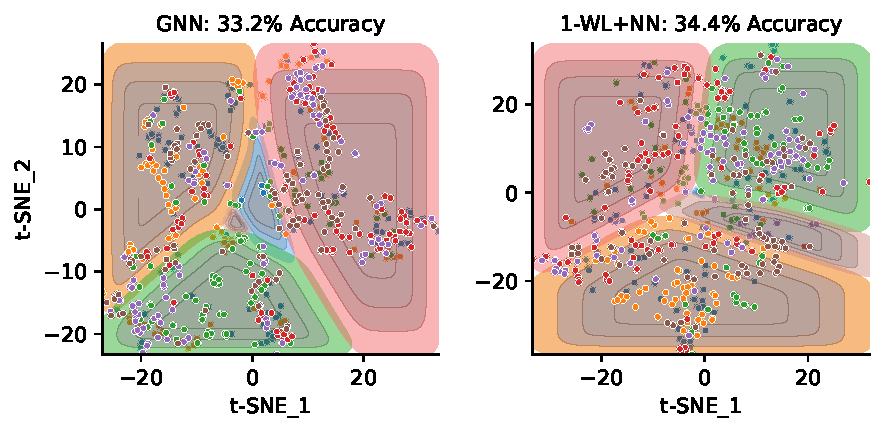
\includegraphics[width=\textwidth]{Figures/tsne_svm_lin_ENZYMES.pdf}
		\vspace*{-4ex} 
		\caption{\enzymes}
	\end{subfigure}
	\hfill
	\begin{subfigure}[b]{0.49\textwidth}
		\centering
		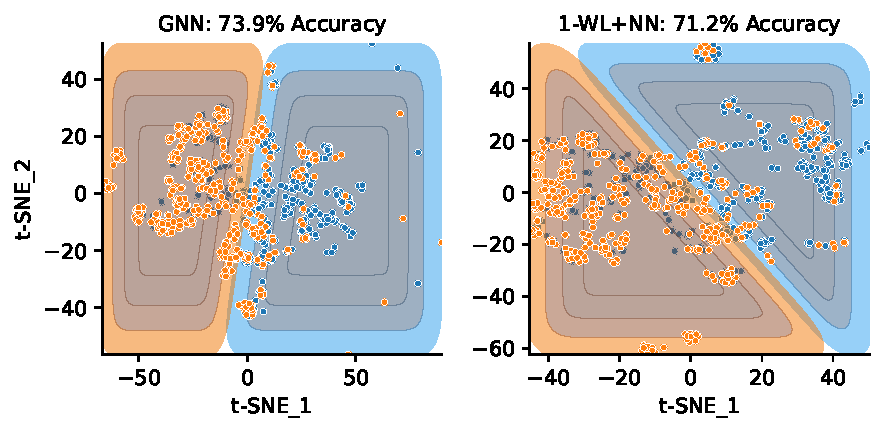
\includegraphics[width=\textwidth]{Figures/tsne_svm_lin_IMDB.pdf}
		\vspace*{-4ex} 
		\caption{\imdb}
	\end{subfigure}
	\par\bigskip
	\begin{subfigure}[b]{0.49\textwidth}
		\centering
		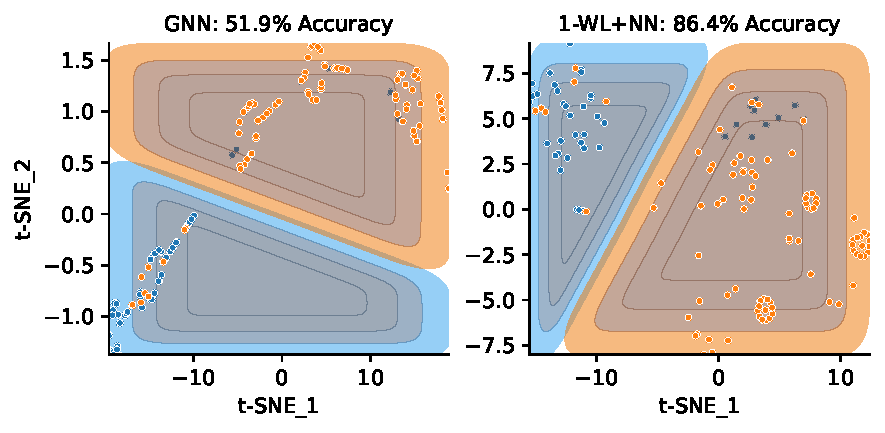
\includegraphics[width=\textwidth]{Figures/tsne_svm_lin_MUTAG.pdf}
		\vspace*{-4ex} 
		\caption{\mutag}
	\end{subfigure}
	\hfill
	\begin{subfigure}[b]{0.49\textwidth}
		\centering
		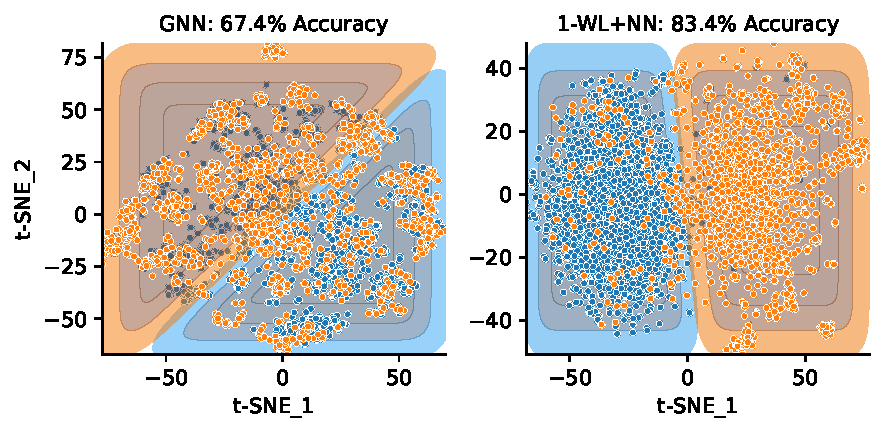
\includegraphics[width=\textwidth]{Figures/tsne_svm_lin_NCI1.pdf}
		\vspace*{-4ex} 
		\caption{\nci}
	\end{subfigure}
	\par\bigskip
	\begin{subfigure}[b]{0.49\textwidth}
		\centering
		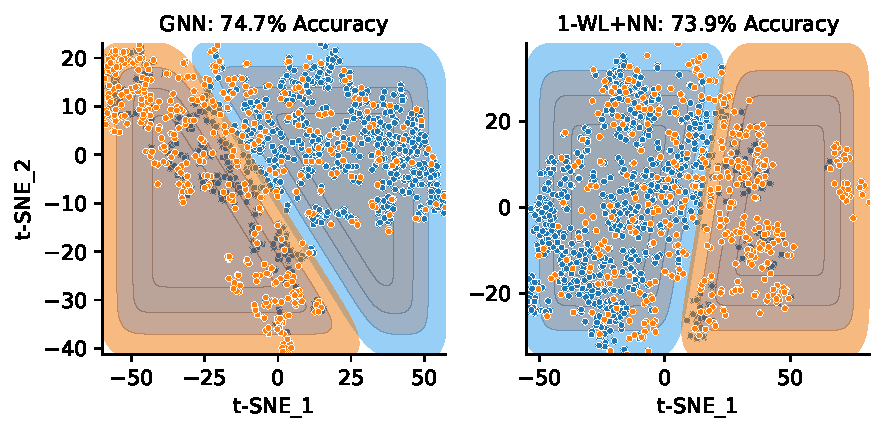
\includegraphics[width=\textwidth]{Figures/tsne_svm_lin_PROTEINS.pdf}
		\vspace*{-4ex} 
		\caption{\proteins}
	\end{subfigure}
	\hfill
	\begin{subfigure}[b]{0.49\textwidth}
		\centering
		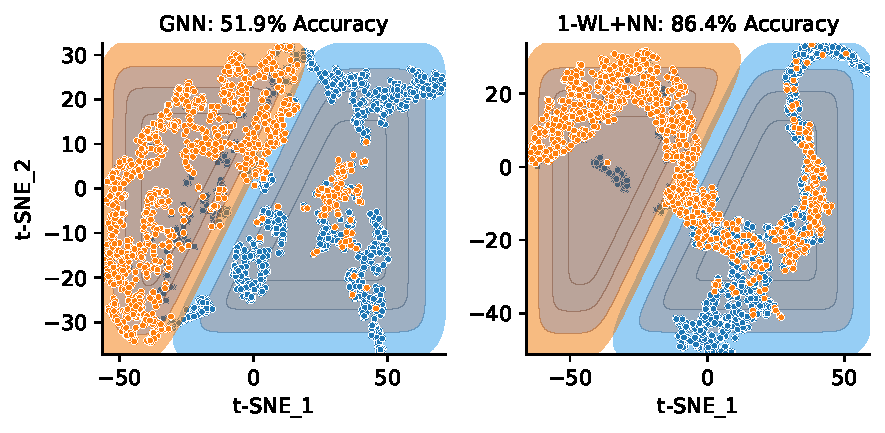
\includegraphics[width=\textwidth]{Figures/tsne_svm_lin_REDDIT.pdf}
		\vspace*{-4ex} 
		\caption{\reddit}
	\end{subfigure}
	\caption{Visualization of the decision boundary of each \textsf{SVM Linear} using \textsf{t-SNE} for the reduction of the dimensionality to two dimensions.}
	\label{fig:pool_svm_tsne}
\end{figure}

For a visualization of the decision boundary calculated by \textsf{SVM Linear}, see \cref{fig:pool_svm_tsne}. We used the \textsf{t-distributed stochastic neighbor embedding (t-SNE)} to reduce the dimensions of the graph representation for visualization purposes. However, note that the \textsf{t-SNE} method distorts the actual distances between data points, such that these visualizations only aid the imagination of the actual relation between graph representations. 

The insight that the \gnn and the \wlnn model compute node representations that, when pooled into a single graph representation, allow for good linear separability further support our  hypothesis that the extra expressiveness contained in the \wl colorings is unnecessary, and \gnns indeed employ a more efficient encoding, as suggested in the previous section.

Another interesting property we also want to investigate is how well these graph representations cluster in their high dimensional space with respect to their class label. To do so, we utilized the \textsf{$k$-NN} classifier for different values of $k$ with $k$ ranging from $1$ to $200$ (except for the \mutag dataset, which only contains 188 graphs, $k$ was limited to a range of $1$ to $150$). Our primary interest was to observe if any range of $k$ values exists where the accuracy consistently remained high. The existence of such a range indicates the presence of meaningful clusters among all graph representations. In order to observe such patterns, we plotted the accuracy achieved on each dataset against the corresponding $k$ values, as illustrated in \cref{fig:pool_knn}.

\begin{figure}[!htb]
	\begin{subfigure}[b]{0.3\textwidth}
		\centering
		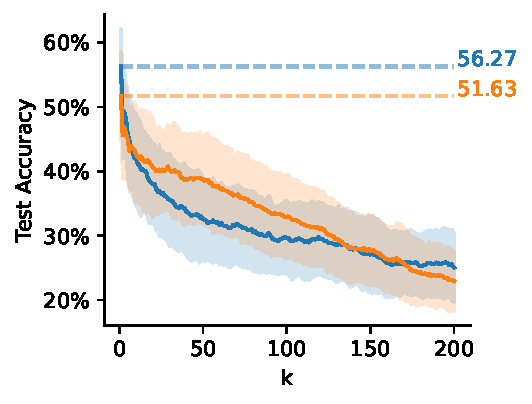
\includegraphics[width=\textwidth]{Figures/knn_ENZYMES.pdf}
		\vspace*{-4ex} 
		\caption{\enzymes}
	\end{subfigure}
	\hfill
	\begin{subfigure}[b]{0.3\textwidth}
		\centering
		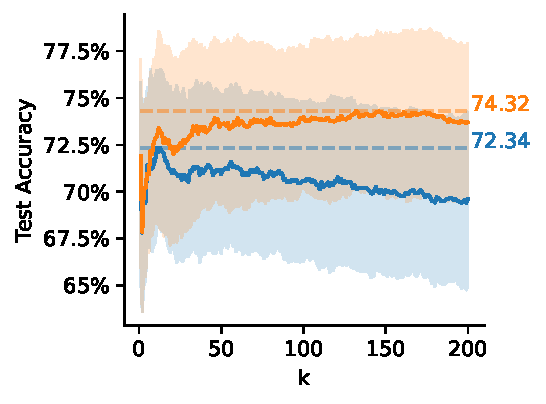
\includegraphics[width=\textwidth]{Figures/knn_IMDB-BINARY.pdf}
		\vspace*{-4ex} 
		\caption{\imdb}
	\end{subfigure}
	\hfill
	\begin{subfigure}[b]{0.3\textwidth}
		\centering
		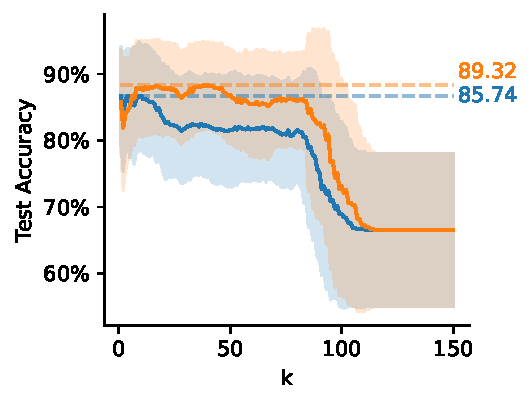
\includegraphics[width=\textwidth]{Figures/knn_MUTAG.pdf}
		\vspace*{-4ex} 
		\caption{\mutag}
	\end{subfigure}
	\par\bigskip
	\begin{subfigure}[b]{0.3\textwidth}
		\centering
		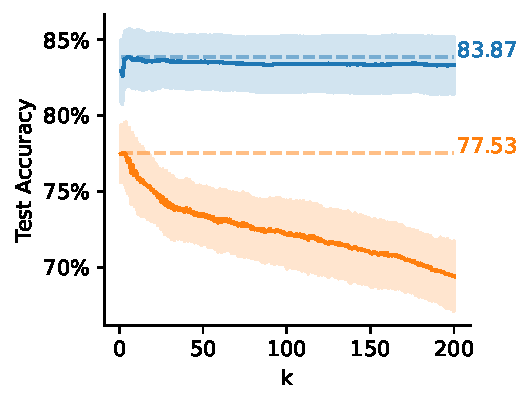
\includegraphics[width=\textwidth]{Figures/knn_NCI1.pdf}
		\vspace*{-4ex} 
		\caption{\nci}
	\end{subfigure}
	\hfill
	\begin{subfigure}[b]{0.3\textwidth}
		\centering
		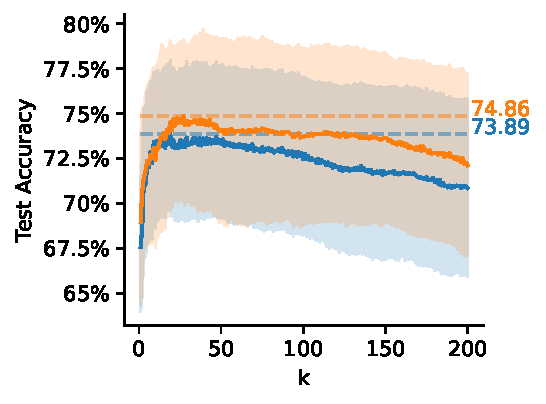
\includegraphics[width=\textwidth]{Figures/knn_PROTEINS.pdf}
		\vspace*{-4ex} 
		\caption{\proteins}
	\end{subfigure}
	\hfill
	\begin{subfigure}[b]{0.3\textwidth}
		\centering
		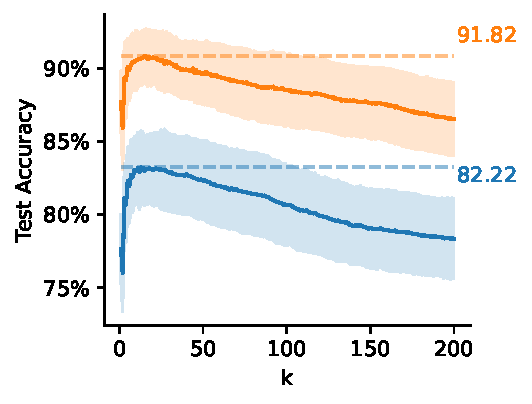
\includegraphics[width=\textwidth]{Figures/knn_REDDIT-BINARY.pdf}
		\vspace*{-4ex} 
		\caption{\reddit}
	\end{subfigure}
	\centering
	\begin{subfigure}[b]{0.3\textwidth}
		\centering
		
\includegraphics[width=\textwidth]{Figures/train_test_diff_legend.pdf}
		\vspace*{-4ex} 
	\end{subfigure}
	\caption{Average classification accuracy achieved on each dataset by replacing the multilayer perceptron of the best-performing \wlnn and \gnn model with a classifier based on the $k$-nearest neighbors algorithm. We tested for different values of $k$.}
	\label{fig:pool_knn}
\end{figure}

Interestingly we can see for all datasets that for some range of $k$ values, there exists a sort of plateau of the accuracy curve, except for the \enzymes and \nci datasets. These plateaus corresponded to the highest accuracy achieved among all $k$ values, indicating that both graph representations computed by \wlnn and \gnn models indeed form meaningful clusters with respect to their class labels. Furthermore, as the \gnn model outperformed the \wlnn model for most $k$ values, we can conclude that the higher expressiveness of the node representation comnputed by the \wl algorithm is obsolete and the \gnn models indeed compute a more efficient encoding of its nodes, which leads to pooled graph representations that achieved the same or even better results in terms of clustering. This insight is even more pronounced in the example of the \reddit dataset, as here, a significant difference exists in its clustering behavior compared to the \wlnn models.

In the case of the \enzymes dataset, allthough there is exist no such a platue, the accuracy achievable on the graph representions is for both types of models very similiar, such that the lack of indication for clustering can probaly be attributed to the dataset itself.

In the case of the \enzymes dataset, while there is no clear plateau in the curve, the accuracy achievable on the graph representations is very similar for both types of models, indicating that the lack of a distinct clustering indication may be attributed to the characteristics of the dataset.

The real exception, however, lies in the behavior of the \textsf{$k$-NN} when applied to the \nci dataset. Here, only the graph representations computed by the \wlnn model exhibit strong clustering performance that remains consistently high across all values of $k$. In contrast, the graph representations of the \gnn model do not seem to cluster at all, and the maximum achievable accuracy is significantly lower than the average accuracy achieved by the \wlnn model representations. We attribute this effect to the \wlnn model's use of three iterations of the \wl algorithm, compared to just one iteration used by all other models of the other datasets. Since the \nci dataset encodes essential information for solving its respective task structurally, this pattern might only be specific to this dataset. Moreover, we observed that no other dataset showed better performance of its \wlnn models with an increased number of \wl iterations, as evident in \cref{fig:k_wl_dependence}.

In conclusion, our findings indicate that the pooled graph representations computed by both \wlnn and \gnn models are highly linearly separable in their high-dimensional space while also forming meaningful clusters with respect to their class labels. Notably, the \gnn models demonstrated superior clustering performance, providing further support for our hypothesis that the message-passing layers of a \gnn encode essential information without overly emphasizing expressiveness. This suggests that the \gnn models strike a balance between efficient encoding and required expressiveness depending on their application.


\FloatBarrier
\subsection{Preprocessing Data for \gnns}
As already outlined at the beginning of this section, is that in comparison to all configurations we tested for \wlnn and \gnn models, the best accuracy achieved on all classification datasets is by a \wlnn model, with the clear exception for the \imdb and \reddit dataset. What makes this observation so interesting is that both datasets are the only ones lacking node features, such that we initialize all \gnn models working on them with an encoding of their node degrees. This difference raises the question of whether \gnn models generally perform better when their input graphs undergo preprocessing. Specifically, we aimed to explore if \gnn models achieve improved performance when their graphs are preprocessed using the \wl algorithm for a single iteration. We will refer to such \gnn models as \wl:\gnn.

This idea seems promising as most of the best-performing \wlnn models also utilize a single iteration of the \wl algorithm as their basis for computation. Further, we know that a \wl:\gnn model can already achieve the same accuracy as each \wlnn model by simply forwarding the preprocessed input graph to the pooling function. However, we hope that \wl:\gnn models leverage their message-passing layers to generate an improved node representation, ultimately leading to enhanced performance in the end.

We conducted the same hyperparameter optimization routines as for the normal \gnn models and listed the classification accuracy achieved by the best-performing configuration of a \wl:\gnn model for each dataset in Table 8. We also included the best performances of each \wlnn and \gnn models for comparison. However, it is essential to note that due to the time constraints of this work and the prioritization of hyperparameter optimization for \gnn and \wlnn models, we tested fewer configurations for \wl:\gnn models. Consequently, these results should be interpreted with caution.

\begin{table}[!htb]
	\caption{Overview of the classification accuracies achieved by the best model configuration for each dataset in percent and standard deviation. Additionally, the performance of each configuration was furhter evaluated by substituting the final \mlp with either a \textsf{SVM} utilizing a linear kernel (\textsf{SVM Linear}) or the Radial Basis Function (\textsf{SVM RBF}), as well as the \textsf{$k$-NN} classifier with different values for $k$.}
	\label{tab:wlnn_gnn}
    \resizebox{.975\textwidth}{!}{ 	\renewcommand{\arraystretch}{1.05}
		\begin{tabular}{@{}c <{\enspace}@{}lcccccc@{}}	\toprule
			& \multirow{3}{*}{\vspace*{4pt}\textbf{Model}}&\multicolumn{6}{c}{\textbf{Dataset}}\\\cmidrule{3-8}
			& & {\enzymes}         &  {\imdb}      & {\mutag}           & {\nci}       & {\proteins}           & 
			{\reddit}
			\\
			\toprule
			\multirow{3}{*}{}
			& \wlnn & 48.3 \scriptsize $\pm 8.1$ & 72.4 \scriptsize $\pm 4.1$ & 85.1 \scriptsize $\pm 8.6$ & 83.6 \scriptsize $\pm 2.2$ & 75.2 \scriptsize $\pm 3.9$ & 78.4 \scriptsize $\pm 2.7$
			\\
			& \wl:\gnn & 35.9 \scriptsize $\pm 6.9$ & 72.0 \scriptsize $\pm 4.1$ & 83.9 \scriptsize $\pm 11.0$ & NaN & 74.5 \scriptsize $\pm 4.1$ &	84.3 \scriptsize $\pm 2.8$
			\\
			& \gnn & 34.4 \scriptsize $\pm 7.0$ & 74.7 \scriptsize $\pm 3.8$ & 84.6 \scriptsize $\pm 8.7$ & 79.9 \scriptsize $\pm 2.2$ & 74.3 \scriptsize $\pm 5.1$ & 86.9 \scriptsize $\pm 3.2$
			\\
			\bottomrule
		\end{tabular}}            
\end{table}
Upon analyzing the best accuracies achieved by each \wl:\gnn model in comparison to the other model types, we observed that its performance is not significantly better than any of the \gnn or \wlnn models. While it does show minor improvements compared to the \gnn models, such as in the \enzymes and \proteins datasets, these improvements are not significant. However, it is important to note that the number of runs conducted for \wl:\gnn models, 143 runs in total, is considerably smaller compared to the 5\,422 runs conducted for \wlnn models and 1\,043 runs for \gnn models. As a result, the limited number of runs might have impacted the statistical robustness of the results. For a full list of the number of runs condcuted, refer to \cref{tab:num_runs} in the Appendix. Further investigation with a larger number of runs could provide more conclusive insights into the performance of \wl:\gnn models.

\FloatBarrier
\subsection{Size of datasets}
Another improtant observation, similiar to our analysis of why \wlnn models with higher number of \wl iterations fail to generalize. Even by fixing the number of \wl iterations to one, \wlnn models still do not scale well for very large datasets. This

Reddit 3032 -> many colors
Regresson datasets

\FloatBarrier
\section{Discusssion}\label{sec:discussion}
\begin{itemize}
	\item \wlnn is a very good tool for investigating \gnns
	\begin{itemize}
		\item many imperical simalarities
	\end{itemize}
\end{itemize}

\subsection{Learned Lessons}
\subsection{Future Work}

\section{Conclusion}

\newpage


